\documentclass[zihao = -4, linespread = 1.5]{article}

\usepackage[heading = true]{ctex}
\usepackage[bottom]{footmisc}
\usepackage[table]{xcolor}
\usepackage{bm}
\usepackage{tikz}
\usepackage{xeCJK}
\usepackage{float}
\usepackage{natbib}
\usepackage{pifont}
\usepackage{datetime}
\usepackage{geometry}
\usepackage{booktabs}
\usepackage{pdfpages}
\usepackage{fancyhdr}
\usepackage{hyperref}
\usepackage{graphicx}
\usepackage{multirow}
\usepackage{multicol}
\usepackage{makecell}
\usepackage{enumitem}
\usepackage{setspace}
\usepackage{pgfplots}
\usepackage{listings}
\usepackage{threeparttable}
\usepackage{amsmath, amssymb, amsfonts, mathrsfs}

\newCJKfontfamily\JiangChengXieSongTi{Italic-SimSun.ttf}
\newcommand{\itsongti}[1]{{\JiangChengXieSongTi#1}}

\pgfplotsset{compat = 1.18}
\usepgfplotslibrary{groupplots}

\definecolor{cadetblue}{HTML}{5F9EA0}
\definecolor{deepred}{RGB}{178, 34, 34}
\definecolor{deepblue}{RGB}{40, 115, 180}
\definecolor{darksalmon}{rgb}{0.91, 0.59, 0.48}
\definecolor{forestgreen}{rgb}{0.13, 0.55, 0.13}

\definecolor{grad1}{HTML}{F2E9E4}
\definecolor{grad2}{HTML}{EAE0D5}
\definecolor{grad3}{HTML}{D5DBCB}
\definecolor{grad4}{HTML}{C6D5C5}
\definecolor{grad5}{HTML}{A3B5A5}
\definecolor{grad6}{HTML}{82B0AA}
\definecolor{grad7}{HTML}{66969A}
\definecolor{grad8}{HTML}{4A8B93}
\definecolor{grad9}{HTML}{2A6D79}
\definecolor{grad10}{HTML}{00505F}

\definecolor{mred1}{HTML}{F2EBE9}
\definecolor{mred2}{HTML}{E0C0B8}
\definecolor{mred3}{HTML}{C08E83}
\definecolor{mred4}{HTML}{9E695D}
\definecolor{mred5}{HTML}{6B3E35}

\definecolor{MorandiLightCyan}{RGB}{209, 238, 238}
\definecolor{MorandiBlue}{RGB}{70, 110, 255}
\definecolor{MorandiGrey}{RGB}{80, 100, 100}
\definecolor{MorandiPurple}{RGB}{140, 110, 180}
\definecolor{MorandiCyan}{RGB}{110, 170, 190}
\definecolor{MorandiRed}{RGB}{220, 130, 130}
\definecolor{MorandiOrange}{RGB}{250, 210, 160}

\geometry{
    a4paper,
    top = 2.54cm,
    bottom = 2.1cm,
    left = 2.5cm,
    right = 2.5cm,
    headheight = -1em
}

% \setitemize[1]{
%     itemsep = 0pt,
%     partopsep = 0pt,
%     parsep = \parskip,
%     topsep = 5pt,
%     leftmargin = 2em,
%     labelsep = 0.25em
% }

% \setenumerate[1]{
%     itemsep = 0pt,
%     partopsep = 0pt,
%     parsep = \parskip,
%     topsep = 5pt,
%     leftmargin = 2em,
%     labelsep = 0.25em
% }

\setlist[1]{
    itemsep = 0pt,
    partopsep = 0pt,
    parsep = \parskip,
    topsep = 5pt,
    leftmargin = 2em,
    labelsep = 0.25em
}

\pagestyle{fancy}
\fancyhf{}
\renewcommand{\headrulewidth}{0pt}
\chead{\includegraphics*[scale = 0.1]{./figs/logo.png}}
\renewcommand{\thefootnote}{\textcolor{deepred}{\arabic{footnote}}}
\renewcommand{\footnoterule}{\kern -3pt \hrule width 0.75\textwidth height 0.5pt \kern 3pt}

\newcommand{\upcite}[1]{\textsuperscript{\textsuperscript{\cite{#1}}}}
\bibpunct{(}{)}{;}{a}{\textcolor{deepblue}{,}}{,}

\hypersetup{
    colorlinks = true,
    citecolor = deepblue,
    linkcolor = deepred,
    urlcolor = deepred
}

\newcolumntype{C}[1]{>{\centering\arraybackslash}p{#1}}
\newcolumntype{M}[1]{>{\centering\arraybackslash}m{#1}}

\ctexset{
    section = {
        number = \arabic{section},
        format = \zihao{3}\bfseries\raggedright,
        aftername = \hspace{1em}
    },
    subsection = {
        format = \zihao{-3}\bfseries\raggedright,
        aftername = \hspace{1em}
    },
    subsubsection = {
        format = \zihao{4}\bfseries\raggedright,
        aftername = \hspace{1em}
    }
}

\newcommand{\cube}[1]{
    \begin{tikzpicture}[baseline = 0ex]
        \draw[
            draw = #1,
            fill = #1!20,
            thick,
            rounded corners = 0.5pt
        ] (0,0) rectangle (0.25, 0.25);
    \end{tikzpicture}
}
\newcommand{\barline}[1]{\overline{#1\rule{0pt}{1.5ex}}}
\renewcommand{\d}{\mathrm{d}}



\begin{document}




\includepdf[pages = -]{./figs/cover.pdf}
\clearpage
\thispagestyle{empty}
\centerline{\tt12:05, Wednesday 31$^{\tt st}$ December, 2025 $\rightsquigarrow$ \currenttime,\ \today}
\mbox{}
\begin{spacing}{1.5}
    \tableofcontents
\end{spacing}
\clearpage
\vspace*{12em}

\centerline{\heiti\bfseries\zihao{2}研~究~生~课~程~论~文}
\centerline{\heiti\bfseries\zihao{-3}（正文）}
\vspace*{4.2em}
\centerline{\bfseries\zihao{-2}家庭教育期望对初中生心理健康的影响}
\vspace*{1.8em}
\centerline{\bfseries\zihao{4}Illusionna}
\vspace*{3.2em}

\noindent\textbf{摘要：}本文基于中国教育追踪调查 CEPS 问卷数据集，筛选 6891 名七年级初中生及其家长作为有效样本，系统探究了家庭教育对青少年心理健康的影响及其作用机制。描述性统计显示，当前家庭普遍存在高学历期望，且家长期望高于孩子期望的代际偏差在汉族及男生群体中尤为显著。差异性检验表明，男生、独生子女、家庭经济优渥和拥有独立书桌的学生心理健康水平显著更高，家庭经济对心理健康具有稳健的保障作用。实证分析发现，学生及家长对未来的信心是心理健康最强的正向预测因子，而学业压力则产生显著的负面影响。中介效应检验进一步印证，对未来信心水平在家庭教育期望与青少年心理健康之间起到 42.3\% 的显著中介作用，家长高期望若能转化孩子自信，将有效促进心理健康。建议家长应注重建立基于信任的支持而非单纯的施压要求，致力于减小亲子期望偏差，关注经济困难家庭学生心理资源建设，以促进青少年身心健康发展。

\vspace*{1em}

\noindent\textbf{关键词：}青少年心理健康；家庭教育期望；学业压力；中介效应


\clearpage
\chead{}
\cfoot{\thepage}
\setcounter{page}{1}



\section{引言}
百年大计，教育为本。党中央的二十大报告中明确指出：“教育、科技、人才是全面建设社会主义现代化国家的基础性、战略性支撑。必须坚持科技是第一生产力、人才是第一资源、创新是第一动力，深入实施科教兴国战略、人才强国战略、创新驱动发展战略，开辟发展新领域新赛道，不断塑造发展新动能新优势”，这一论断将教育的地位提升到了前所未有的战略高度，论断充分体现了在新时代新征程中，教育所发挥的基础性、先导性、全局性作用。

我国的现代化教育体系中，教育不再仅局限于学校课题之中，更多时候演变成一个深度卷入家庭、社会及国家竞争的复合场域。作为教育体系的重要组成部分，青少年家庭教育是学校教育和社会教育的基础起点，因此在新时代背景下，如何办好青少年教育已成为家庭、学校和社会的共同责任。此外在党的二十大报告中更进一步强调要“深化教育领域综合改革，加强教材建设和管理，完善学校管理和教育评价体系，健全学校家庭社会育人机制。加强师德师风建设，培养高素质教师队伍，弘扬尊师重教社会风尚。推进教育数字化，建设全民终身学习的学习型社会、学习型大国”，这又标志着协同育人已经从教育理念升华至国家意志，打造出三方合力，形成良性循环的支持系统，共同促进青少年教育的高质量发展。



\section{研究背景与意义}
\subsection{背景}
长期以来，人们认为家庭教育在某种程度上被视为“家事”，其质量参差不齐，缺乏科学的指引。然而现在随着社会对人才培养质量要求的提高，我国家庭教育的地位日益凸显。2021 年 10 月 23 日表决通过《中华人民共和国家庭教育促进法》，并于 2022 年 1 月 1 日正式施行，这一法律的颁布，标志着我国正式进入了“依法教子”的新时代，强调了家长应当树立家庭是第一课堂的责任意识，用正确思想引领、教育方法和行为举止，肩负起青少年子女养成良好思想、品行和习惯的重任，构建成熟教育体系的重要一环。法案明确了家庭教育的特点，即要贯彻科学的家庭教育理念和方法，家长不仅作为青少年孩子的第一任老师，也是子女的终身教师。由于家庭教育具有早期性教育的特点，家长会潜移默化影响青少年孩子，所以国家和社会更应为家庭教育提供指导、支持与服务，保障家庭教育对青少年生活习惯、道德行为、言语意识的正确发展，减少教育焦虑、学生压力这一社会现象。

父母家庭是孩子生命的摇篮，是个体出生后接受到教育的第一站，是青少年子女人生的第一课堂。相比于学校教育和社会教育，家庭教育具有极其独特的逻辑规律：

\begin{itemize}
    \item 早期性与启蒙性：家长是孩子的启蒙老师，家庭教育是青少年个体社会化过程的开端，它不仅影响着学生的生活习惯与道德品行，更在潜移默化中塑造着个体的性格底色；
    \item 连续性与终身性：研究指出，排除睡觉时间，学生在校时间仅占生命前 18 年总时间的小部分，约 $2/3$ 时间在家庭环境中度过~\citep{Walberg}，家庭教育通过家长的一言一行，有意识或无意识地在任何时间、任何地点进行着，这种影响伴随青少年一生，因此家长被称为“终身教师”；
    \item 基础性与全局性：在“学校-家庭-社会”三位一体的教育体系中，家庭教育是青少年心理健康发展的底色，倘若忽视家庭教育的基石作用，不仅会削弱学校教育的成效，甚至可能对青少年心理健康成长造成不可挽回的损伤。
\end{itemize}

尽管我国高度重视家庭教育，但现实中的矛盾依然尖锐。随着知识时代的推进，社会阶层流动的压力日益增大，家庭作为孩子成长的第一阵地，父母教育期望功能被前所未有地强化，具体而言包括：“望子成龙、望女成凤”是传统家庭的普遍期望；2019 年两会期间提出的《关于进一步促进家庭教育发展的提案》中表明 68\% 的家长对青少年子女教育很焦虑；2021 年 7 月 24 日出台的《关于进一步减轻义务教育阶段学生作业负担和校外培训负担的意见》（即“双减”政策）指出家长对青少年子女的期望压力处于深度焦虑之中。

家庭是持续影响青少年个体成长的重要因素，家长父母教育期望是影响子女学业成绩的关键因素，家庭教育期望差异过大很可能造成青少年心理健康问题，产生负面焦虑情绪，最终影响学业成绩~\citep{WangYaNan}，因此本文将进行系统地研究，提供切实可行的策略和建议。



\subsection{意义}
本课程论文研究围绕家庭教育期望和青少年初中生心理健康的影响展开深入探讨，目前的学术研究多集中于教育期望对“学业成绩”的影响，而“心理健康”这一更重要的指标关注欠缺，针对初中生尤其七年级学生这一特定群体，其研究意义不仅在于理论层面的科学逻辑构建，而且更在于为当前转型时期的教育实践提供科学指引，丰富国内青少年教育心理学领域研究空白，解析家庭期望对青少年心理健康的动态数据科学支持。

其一从理论研究深度而言，本研究有助于进一步深化家庭生态系统理论在当今中国社会背景下的应用，虽然国内外有关父母期望与青少年子女学业成就的关系已有丰硕的成果，但家庭内部的期望传递机制对青少年心理健康正发生着深刻的结构性变化。本文通过实证分析，探究家庭教育期望如何通过心理控制、焦虑传播等中介变量影响七年级青少年初中生的心理情绪健康，这样不仅能够丰富青少年心理发展的科学实证数据，而且也能够解释我国本土语境下，一些传统观念对现代化素质教育理念影响，提供新的理论视角，有助于填补七年级学生群体在复杂教育政策环境下的心理轨迹研究空白，构建更具体更学术更具有针对性的青少年心理健康模型。

其二从实践应用层面而言，本文对改善家庭教育质量、提升青少年心理健康教育水平具有直接影响作用，研究结果能够为广大七年级初中生家长提供科学的心理健康画像，帮助鉴别过度教育期望可能带来的“反噬风险”，从而引导家长从盲目追求学业成就转向对子女心理健康需求的关注。通过对研究结论的转化，可以引导家长设定合理的教育目标，建立更具支持下可建设性的亲子关系，缓解亲子冲突，从而在源头上缓解青少年学生学业压力焦虑。

其三从学校教育层面而言，本研究为完善家校协同育人机制提供实证依据，对于广大的教育工作从事者，承担立德树人、情感熏陶的重要使命，本研究将帮助教育工作者针对性地融入青少年心理健康教育，利用人文关怀去抚慰困于家庭教育期望压力下的学生，为教师引导学生心理健康提供了精确的切入点。此外，本研究结论也能为教育行政部门优化“双减”政策，为其提供参考依据，通过缓解家庭期望焦虑，真正实现教育本心回归，让教育由单纯的竞争转向人的全面发展，为青少年心理健康构建更加科学和谐的生态环境，实现心理健康与学业发展的双赢。



\subsection{研究问题内容}
文章依托中国教育追踪调查 CEPS 数据库，重点聚焦于初中七年级青少年学生群体，文章将系统展开关于家庭教育期望与青少年心理健康之间的关系实证分析。

\begin{itemize}
    \item 研究将致力于通过描述性统计分析，呈现当前家庭教育期望分布现状以及青少年心理健康水平特质，本研究将量化分析家长对子女的学历期望、成绩期望在不同社会阶层、不同家庭结构中的具体表现，勾勒出七年级学生在面对家庭教育期望时的心理健康画像，探究家庭内部期望是否已经演变成一种普遍的负面情绪心理焦虑来源，在明确这一直接效应的基础上，利用相关 CEPS 量表，深度探究影响路径，即学业压力是否在家庭教育期望与青少年心理健康之间发挥关键的中介作用，进而剖析外部期望是如何转化为青少年学生内部认知负担并最终损害心理情绪健康；
    \item 研究的核心内容在于深入分析家庭教育期望对青少年七年前初中生心理健康的直接影响机制及其内在逻辑，尽管既往研究多探讨教育期望对“学业成绩”的影响，但本研究将视角转向更为隐性的“心理健康”指标，论文利用 CEPS 数据集建立回归模型，实证检验父母的教育期望是否会对子女产生反噬副作用，即过度的期望差距是否导致青少年交流，在此基础上，进一步引入心理控制、焦虑传播相关的中介变量，解释家庭教育期望是如何通过亲子互动的心理机制传递给青少年子女的，这将有助于填补相关家庭内部期望传递机制对青少年心理健康影响的结构性变化研究空白；
    \item 研究最后是关注家庭教育期望影响效应的异质性分析，探究不同群体中表现的差异性，譬如青少年性别差异、家长性别差异等多个维度展开深入讨论，具体来说就是研究青少年男女心理健康是否存在显著不同，父亲母亲作为不同教育主体，其期望值差异对子女心理健康产业的效应是否具有非对称性，通过多维度细分研究，旨在为不同类型的家庭提供更具针对性的教育指导策略，帮助家长设定合理的教育目标，并且在源头上缓解亲子冲突，为构建家庭协同育人机制提供精准的实证依据，为家长设定合理的期望，最终实现从单纯的学业竞争向关注青少年全面心理健康的教育本心回归。
\end{itemize}



\section{文献综述}
青少年时期是个体身心发展的关键阶段，也是心理健康问题的高发期。据联合国儿童基金会和世界卫生组织报告，全球 12 亿 $10\sim19$ 岁的青少年中，约有 20\% 存在心理健康问题，并且该年龄段的群体所遭受约 16\% 的疾病和伤害是由心理健康问题引起的，大量的研究数据也一致表明，心理健康问题已成为诸多青少年在青春期面临的一个常见问题~\citep{CEPS}。发展心理学家尤里·布朗芬布伦纳提出的生态系统理论中，指明环境对青少年个体影响是系统性的，包括家庭、学校、同龄人等，这是根据环境变化而形成的~\citep{Bronfenbrenner}，因此我们可以观察到家庭作为青少年成长的微观系统，其环境因素对个人发展具有深远影响。其中，父母教育期望作为家庭教育观念的核心要素，被广泛认为是影响青少年学业成绩和心理健康发展的重要变量，然而，现有的研究关于父母教育期望对青少年心理健康的影响结论不完全一致，且亲子间教育期望的互动关系（代际偏差）及其内在作用机制（学业压力、家长投入等）逐渐成为学术界的焦点，本课程论文将从父母教育期望的直接影响、家庭教育期望偏差的效应、相关中介与调节机制等方面对现有文献进行综述。

父母教育期望的定义是指父母对子女未来能够达到的最高教育水平的信念或预期。关于其对青少年心理健康的影响，目前的学术界存在“积极论”与“消极论”两种主要观点。

一方面，部分学者认为高期望是青少年心理发展的保护性因素，基于 CEPS 数据集的研究发现，父母较高的教育期望与青少年较少的心理健康问题相关，高期望往往伴随着家长对青少年子女未来的信心和支持，能够很好地激发青少年子女的自我效能感和成就动机。随着父母教育期望的提高，青少年的抑郁水平显著降低~\citep{Resnick}，这表明在一定的条件下，高期望可以作为一种积极的心理资源，通过提供目标导向，促进青少年的心理健康适应。

另一方面，更多的实证研究指出，高期望的潜在负面影响，即期望异化~\citep{MaBianJing}。在社会文化角度而言，学者们认为亚洲文化深受儒家哲学影响，家长对青少年子女抱有更高的期望，并且为此投入更多的资金用于孩子学习，还教育子女服从和满足父母的期望需求~\citep{Cultural}，中国家庭强调家族荣誉、家庭孝道、勤奋工作等观念，这些观念被传递给子女，寄予极高的学业期望，可能会给青少年带来巨大的心理健康压力，产生诸多心理健康问题。当这种期望超过青少年子女的实际能力或缺乏相应的资源支持之时，就会转化为巨大的心理压力，导致焦虑、抑郁、自卑、自杀意念，即家长教育期望和青少年的负面情绪之间存在正相关关系~\citep{Role}。此外，自我决定理论认为自主性和胜任感是青少年个体大基本心理需要，家长过高期望可能导致采取严厉的心理控制手段，损害青少年子女的心理需求~\citep{LiDaLin}。

鉴于父母与青少年子女作为独立的个体，其对未来的预期往往并不一致，近年来研究视角逐渐从单一的“家长期望”转向“亲子教育期望偏差”，身份控制理论和自我差异理论为解释期望偏差的影响提供了理论框架，这些理论认为，当个体感知到外部评价如父母期望与自我认同标准如自我期望不一致时，会产生认同困扰和心理压力，进而引发负面情绪~\citep{Higgins}。

实证研究表明，亲子教育期望的一致性对青少年心理健康至关重要，“一致高”的模式通常被认为是最优状态，当父母和子女都持有高教育期望时，家庭内部目标一致，能够促进家庭社会资本有效传递，增加亲子互动和教育投入，从而促进青少年学业成绩和心理健康发展~\citep{YangXue}。其次，“父母期望高于子女期望”的偏差通常产生消极影响，多项研究实证表明，当子女感知到父母期望高于自身期望之时，会体验到更多的学业压力、更高的消极情感（譬如抑郁）和更低的积极情感~\citep{GuoXiaoLin}。这种“向上”的偏差意味着青少年子女认为父母的目标难以实现，从而产生挫败感、倦怠感、习得性无助~\citep{Burnout}。最后，关于“家长期望低于子女期望”的影响存在争议，部分研究认为这种偏差可能暗示父母对子女缺乏信心，从而不利于心理健康，但也有研究发现，适度“向下”的期望落差可能为青少年创造相对宽松的环境，使其在自主驱动下获得更好的心理健康状态。值得注意的是，亲子期望偏差与负面情绪之间并非简单的线性关系，只有当偏差达到极端程度时，青少年风险威胁情绪会显著增加~\citep{LiWenZhe}。

深入理解家庭教育期望如何影响心理健康，学者们引入了多种中介和调节变量，构建更为复杂的动态模型。诸多研究表明学业压力在家长期望与青少年心理健康之间起中介作用，当父母期望过高，会加剧子女学业压力，进而导致学业倦怠和抑郁情绪，家长学业压力正向预测青少年的学业抽离，并通过表现回避目标取向产生消极影响~\citep{ZhangYunYun}。

家长投入是连接青少年子女期望与结果的桥梁，一方面高教育期望可以促进家长增加教育投入，例如辅导作业、购买资料，这种通常被视为积极的因素，能降低子女的学业倦怠~\citep{LiRuoXuan}，“一致高”的期望模式下，家长投入能有效传递家庭资本，促进青少年发展，过高期望的父母可能异化青少年子女心理健康，破坏孩子心理需求，导致“依从性”而非“自主性”的学习行为。

并非所有面对高期望或者压力的青少年都会出现心理健康问题，个体自身的心理资源起到了关键的缓冲作用。自我韧性可以调节学业压力对心理适应的影响，高韧性的青少年在面对家长施加的学业成绩压力之时，表现出更少的抑郁和问题行为~\citep{XiongMingLing}，这种自我韧性作为个体心理健康的保护性资源，能够帮助青少年在压力情境下恢复心理平衡~\citep{Burnout}。加之，学业成绩的自我效能感在亲子期望偏差与情感幸福之家起到中介作用，当青少年子女感知到父母期望高于自身时，其学业成绩可能受损，进而降低学业自我效能感，最终导致积极情感减少。

家庭结构和社会经济地位显著调节了教育期望的影响模式，多子女家庭资源会被分散，但也有研究指出非独生子女具有更高的亲社会性~\citep{ChengYaWen}，研究发现，独生子女家庭的父母教育期望普遍高于非独生子女家庭，独生子女家庭中家长更重视孩子的学业成绩和未来发展，因此孩子的表现更好，但在心理健康方面两者无显著差异~\citep{Differences}。

家长学历与家庭阶层方面，高学历或者精英家庭通过投入高质量的亲子互动方式，实现教育期望的协同效应，而普通家庭可能更多依赖增加补习这样的方式进行补偿，但也更容易陷入“内卷化”的负面循环之中~\citep{WangJianWu}。同时，对于成绩较好的学生，高学历父母的过高期望反而可能削弱其学业表现的积极影响~\citep{LiJiaZhe}，产生“天花板边际效应”~\citep{Tichenor}，家长的高学历本身容易给青少年子女带来无形的标签压力，青少年子女内心渴望达到与父母相同的甚至更高的学历，自我期待较高。

综上所述，家长教育期待对青少年初中生子女的心理健康影响具有复杂性，虽然高期望在理想状态下能促进发展，但在现实情境中，尤其是出现家长期望远高于青少年孩子的代际偏差时，往往通过增加学业压力，引发父母心理控制，降低自我效能感等路径，最终对青少年初中生心理健康造成负面影响，不利于实现初中生心理健康的全面发展。



\section{研究方法设计}
\subsection{数据集}
本课程论文研究使用的数据集来源于中国教育追踪调查 CEPS，逗号分隔值 CSV 数据集见 CC0 公有域~\footnote{\href{https://www.kaggle.com/datasets/illusionna/ceps-dataset}{https://www.kaggle.com/datasets/Illusionna/ceps-dataset}}，它是由中国人民大学设计与实施的，具有我国代表性的大型追踪调查项目。该调查以初中一年级和初中三年级，即 7 年级和 9 年级两个群体为调查起点，收集了包括青少年学生、家长、教师、学校等多维度的详细数据。本课程研究只关注七年级青少年初中生及其家庭教育期望对心理健康产生的影响。



\subsection{被试}
CEPS 数据集采用了概率与规模成比例（PPS）的多阶段抽样方法，在全国抽取 28 个县级单位，包括区、县、市，共计 112 所学校，有 438 个班级，共 19487 名青少年初中生，更详尽的抽样设计参考项目源地址~\footnote{\href{https://www.cnsda.org/index.php?r=projects/view&id=72810330}{https://www.cnsda.org/index.php?r=projects/view\&id=72810330}}，我们只研究七年级的初中生，因此忽略全体九年级的学生群体，因此，各有 10279 名学生和家长。



\subsection{研究对象}
为了保证研究结果的准确性，本研究对原始数据进行了以下筛选与处理：首先，剔除全体九年级学生，形成 $10279\times2$ 的青少年学生和家长的样本量；其次，我们重点关注表~\ref{table-variable} 这些维度；最后，对于数据集缺失值，选择直接抛弃该样本，包括学生及其家长，统计结果见表~\ref{table-missing} 所示。通过学生与家长唯一标志符“ids”，求取共同的交集部分，经过严格筛选处理，最终纳入有效的样本量共计 $\bm{6891\times2}$ 个，这些数据样本将用于实证分析。

针对二分类变量，约定赋值：性别中，1 代表男性，0 代表女性；独生子女中，1 代表是独生子女，0 代表不是独生子女；独立书桌中，1 代表有桌子，0 代表无桌子；报辅导班中，1 代表申报，0 代表没有申报；低保中，1 代表领取低保，0 代表不领取低保。

针对量级型变量，约定赋值：$1,\ 2,\ 3,\ \ldots$ 其中 1 代表等级最低或者程度最弱，数字越大，等级与高或程度越强。

针对多分类变量，约定赋值：民族中，1 代表汉，2 代表蒙，3 代表满，4 代表回，5 代表藏，6 代表壮，7 代其他；家长身份中，1 代表生父，2 代表生母，3 代表继父，4 代表继母，5 代表（外）祖父，6 代表（外）祖母，7 代表其他男性亲属，8 代表其他女性亲属，9 代表其他男性非亲属，10 代表其他女性非亲属；意见不一致的解决方法中，1 代表大多顺着孩子，2 代表说服孩子接受您的意见，3 代表强迫孩子接受您的意见，4 代表讨论后看谁有道理就听谁的意见，5 代表不了了之，6 代表其他。

\begin{table}[htbp]
    \centering
    \setlength{\tabcolsep}{16pt}
    \renewcommand{\arraystretch}{1}
    \caption{CEPS 数据集核心研究维度（\textcolor{forestgreen}{\ding{51}} 代表是二分类题）}\label{table-variable}
    \begin{tabular}{cc|cc}
        \bottomrule[1.5pt]
        \rowcolor{cadetblue!20} \multicolumn{2}{c|}{\textbf{学生}} & \multicolumn{2}{c}{\textbf{家长}} \\
        \rowcolor{cadetblue!20} \textbf{变量} & \textbf{解释} & \textbf{变量} & \textbf{解释} \\
        \hline
        a01~\textcolor{forestgreen}{\ding{51}} & 性别 & ba01~\textcolor{darksalmon}{\ding{55}} & 是孩子的什么人 \\
        \rowcolor{gray!10} a03~\textcolor{darksalmon}{\ding{55}} & 民族 & ba02~\textcolor{forestgreen}{\ding{51}} & 本学期是否报辅导班 \\
        a17~\textcolor{darksalmon}{\ding{55}} & 现在的整体健康情况 & ba08~\textcolor{darksalmon}{\ding{55}} & 这些方面管得严不严 \\
        \rowcolor{gray!10} b01~\textcolor{forestgreen}{\ding{51}} & 是否为独生子女 & ba09~\textcolor{darksalmon}{\ding{55}} & 意见不一致时的做法 \\
        b06~\textcolor{darksalmon}{\ding{55}} & 妈妈的教育水平 & ba14~\textcolor{darksalmon}{\ding{55}} & 是否主动与孩子讨论事情 \\
        \rowcolor{gray!10} b07~\textcolor{darksalmon}{\ding{55}} & 爸爸的教育水平 & ba17~\textcolor{darksalmon}{\ding{55}} & 从事活动的频率 \\
        b09~\textcolor{darksalmon}{\ding{55}} & 家庭经济条件 & ba18~\textcolor{darksalmon}{\ding{55}} & 望孩子读到什么程度 \\
        \rowcolor{gray!10} b11~\textcolor{forestgreen}{\ding{51}} & 是否有独立的书桌 & ba21~\textcolor{darksalmon}{\ding{55}} & 对孩子未来是否有信心 \\
        b25~\textcolor{darksalmon}{\ding{55}} & 和父母的关系 & bc10~\textcolor{darksalmon}{\ding{55}} & 孩子目前成绩在班里处于 \\
        \rowcolor{gray!10} b29~\textcolor{darksalmon}{\ding{55}} & 父母为你做的多吗 & bc11~\textcolor{darksalmon}{\ding{55}} & 对孩子成绩要求 \\
        b30~\textcolor{darksalmon}{\ding{55}} & 父母对你学业成绩要求 & bd13~\textcolor{darksalmon}{\ding{55}} & 孩子现在身体健康情况 \\
        \rowcolor{gray!10} b31~\textcolor{darksalmon}{\ding{55}} & 父母对你的教育期望 & be02~\textcolor{darksalmon}{\ding{55}} & 民族 \\
        b32~\textcolor{darksalmon}{\ding{55}} & 对这种期望感到 & be07~\textcolor{darksalmon}{\ding{55}} & 教育程度 \\
        \rowcolor{gray!10} b35~\textcolor{darksalmon}{\ding{55}} & 父母对你未来有信心吗 & be19~\textcolor{darksalmon}{\ding{55}} & 家庭经济条件 \\
        c12~\textcolor{darksalmon}{\ding{55}} & 目前成绩在班里处于 & be20~\textcolor{forestgreen}{\ding{51}} & 是否领取低保 \\
        \rowcolor{gray!10} c22~\textcolor{darksalmon}{\ding{55}} & 自己希望读到什么程度 & - & - \\
        c25~\textcolor{darksalmon}{\ding{55}} & 对自己未来有没有信心 & - & - \\
        \toprule[1.5pt]
    \end{tabular}
\end{table}

\begin{table}[!t]
    \centering
    \setlength{\tabcolsep}{8pt}
    \renewcommand{\arraystretch}{0.75}
    \caption{学生与家长数据集缺失值统计}\label{table-missing}
    \begin{tabular}{ccc|ccc}
        \bottomrule[1.5pt]
        \multicolumn{3}{c|}{\textbf{学生数据集}} & \multicolumn{3}{c}{\textbf{家长数据集}} \\
        \textbf{维度} & \textbf{缺失} & \textbf{占比} & \textbf{维度} & \textbf{缺失} & \textbf{占比} \\
        \hline
        a01   & 196 & 1.91\% & ba01   & 265 & 2.58\% \\
        a03   & 35  & 0.34\% & ba02   & 277 & 2.69\% \\
        a17   & 115 & 1.12\% & ba0801 & 295 & 2.87\% \\
        b01   & 2   & 0.02\% & ba0802 & 399 & 3.88\% \\
        b06   & 230 & 2.24\% & ba0803 & 375 & 3.65\% \\
        b07   & 243 & 2.36\% & ba0804 & 418 & 4.07\% \\
        b09   & 555 & 5.40\% & ba0805 & 373 & 3.63\% \\
        b11   & 282 & 2.74\% & ba0806 & 381 & 3.71\% \\
        b2501 & 58  & 0.56\% & ba0807 & 425 & 4.13\% \\
        b2502 & 60  & 0.58\% & ba0808 & 345 & 3.36\% \\
        b29   & 27  & 0.26\% & ba09   & 286 & 2.78\% \\
        b30   & 70  & 0.68\% & ba1401 & 359 & 3.49\% \\
        b31   & 92  & 0.90\% & ba1402 & 392 & 3.81\% \\
        b32   & 80  & 0.78\% & ba1403 & 390 & 3.79\% \\
        b35   & 43  & 0.42\% & ba1404 & 418 & 4.07\% \\
        c12   & 62  & 0.60\% & ba1405 & 384 & 3.74\% \\
        c22   & 97  & 0.94\% & ba1701 & 413 & 4.02\% \\
        c25   & 104 & 1.01\% & ba1702 & 531 & 5.17\% \\
        -     & -   & -      & ba1703 & 511 & 4.97\% \\
        -     & -   & -      & ba1704 & 647 & 6.29\% \\
        -     & -   & -      & ba1705 & 538 & 5.23\% \\
        -     & -   & -      & ba1706 & 478 & 4.65\% \\
        -     & -   & -      & ba18   & 289 & 2.81\% \\
        -     & -   & -      & ba21   & 294 & 2.86\% \\
        -     & -   & -      & bc10   & 276 & 2.69\% \\
        -     & -   & -      & bc11   & 329 & 3.20\% \\
        -     & -   & -      & bd13   & 445 & 4.33\% \\
        -     & -   & -      & be02   & 368 & 3.58\% \\
        -     & -   & -      & be07   & 388 & 3.77\% \\
        -     & -   & -      & be19   & 363 & 3.53\% \\
        -     & -   & -      & be20   & 552 & 5.37\% \\
        \hline
        \textbf{学生样本} & $10279\rightarrow8650$ & \textbf{剔除 1629} & \textbf{家长样本} & $10279\rightarrow8039$ & \textbf{剔除 2240} \\
        \toprule[1.5pt]
    \end{tabular}
\end{table}



\subsection{研究工具}
\subsubsection{家庭教育期望量表}
家长教育期望是指家长对子女未来学业成就的预期高度，即对 b31 维度进行测量，其中部分数字越大代表家长期望学历级别越高，具体如下：

\begin{center}
    \begin{minipage}{0.9\textwidth}
        \setlength{\columnsep}{2em}
        \setlength{\columnseprule}{0.5pt}
        \begin{multicols}{3}
            \begin{enumerate}
                \item 现在就不要念了
                \item 初中毕业
                \item 中专或技校
                \item 职业高中
                \item 普通高中
                \item 大学专科
                \item 大学本科
                \item 研究生
                \item 博士
                \item 无所谓
            \end{enumerate}
        \end{multicols}
    \end{minipage}
\end{center}



\subsubsection{心理健康量表}
青少年心理健康是指七年级学生当下的整体健康状况，即对 a17 维度进行测量，其中数字值越大代表青少年心理越健康，具体如下：

\begin{center}
    \begin{minipage}{1\textwidth}
        \setlength{\columnsep}{1em}
        \setlength{\columnseprule}{0.5pt}
        \begin{multicols}{5}
            \begin{enumerate}
                \item 很不好
                \item 不太好
                \item 一般
                \item 比较好
                \item 很好
            \end{enumerate}
        \end{multicols}
    \end{minipage}
\end{center}



\subsubsection{学业期望压力中介变量}
本课程研究将学业压力作为核心的中介变量指标，旨在探索外部的家庭期望如何转化为青少年个体的内部认知负担，并最终影响其心理健康，即对 b32 维度进行测量，其中数字越大代表学业压力越强，编号如下：

\begin{center}
    \begin{minipage}{1\textwidth}
        \setlength{\columnsep}{0em}
        \setlength{\columnseprule}{0.5pt}
        \begin{multicols}{5}
            \begin{enumerate}
                \item 毫无压力
                \item 有点压力
                \item 一般
                \item 压力比较大
                \item 压力很大
            \end{enumerate}
        \end{multicols}
    \end{minipage}
\end{center}

\begin{figure}[htbp]
    \centering
    \begin{minipage}{0.48\textwidth}
        \centering
        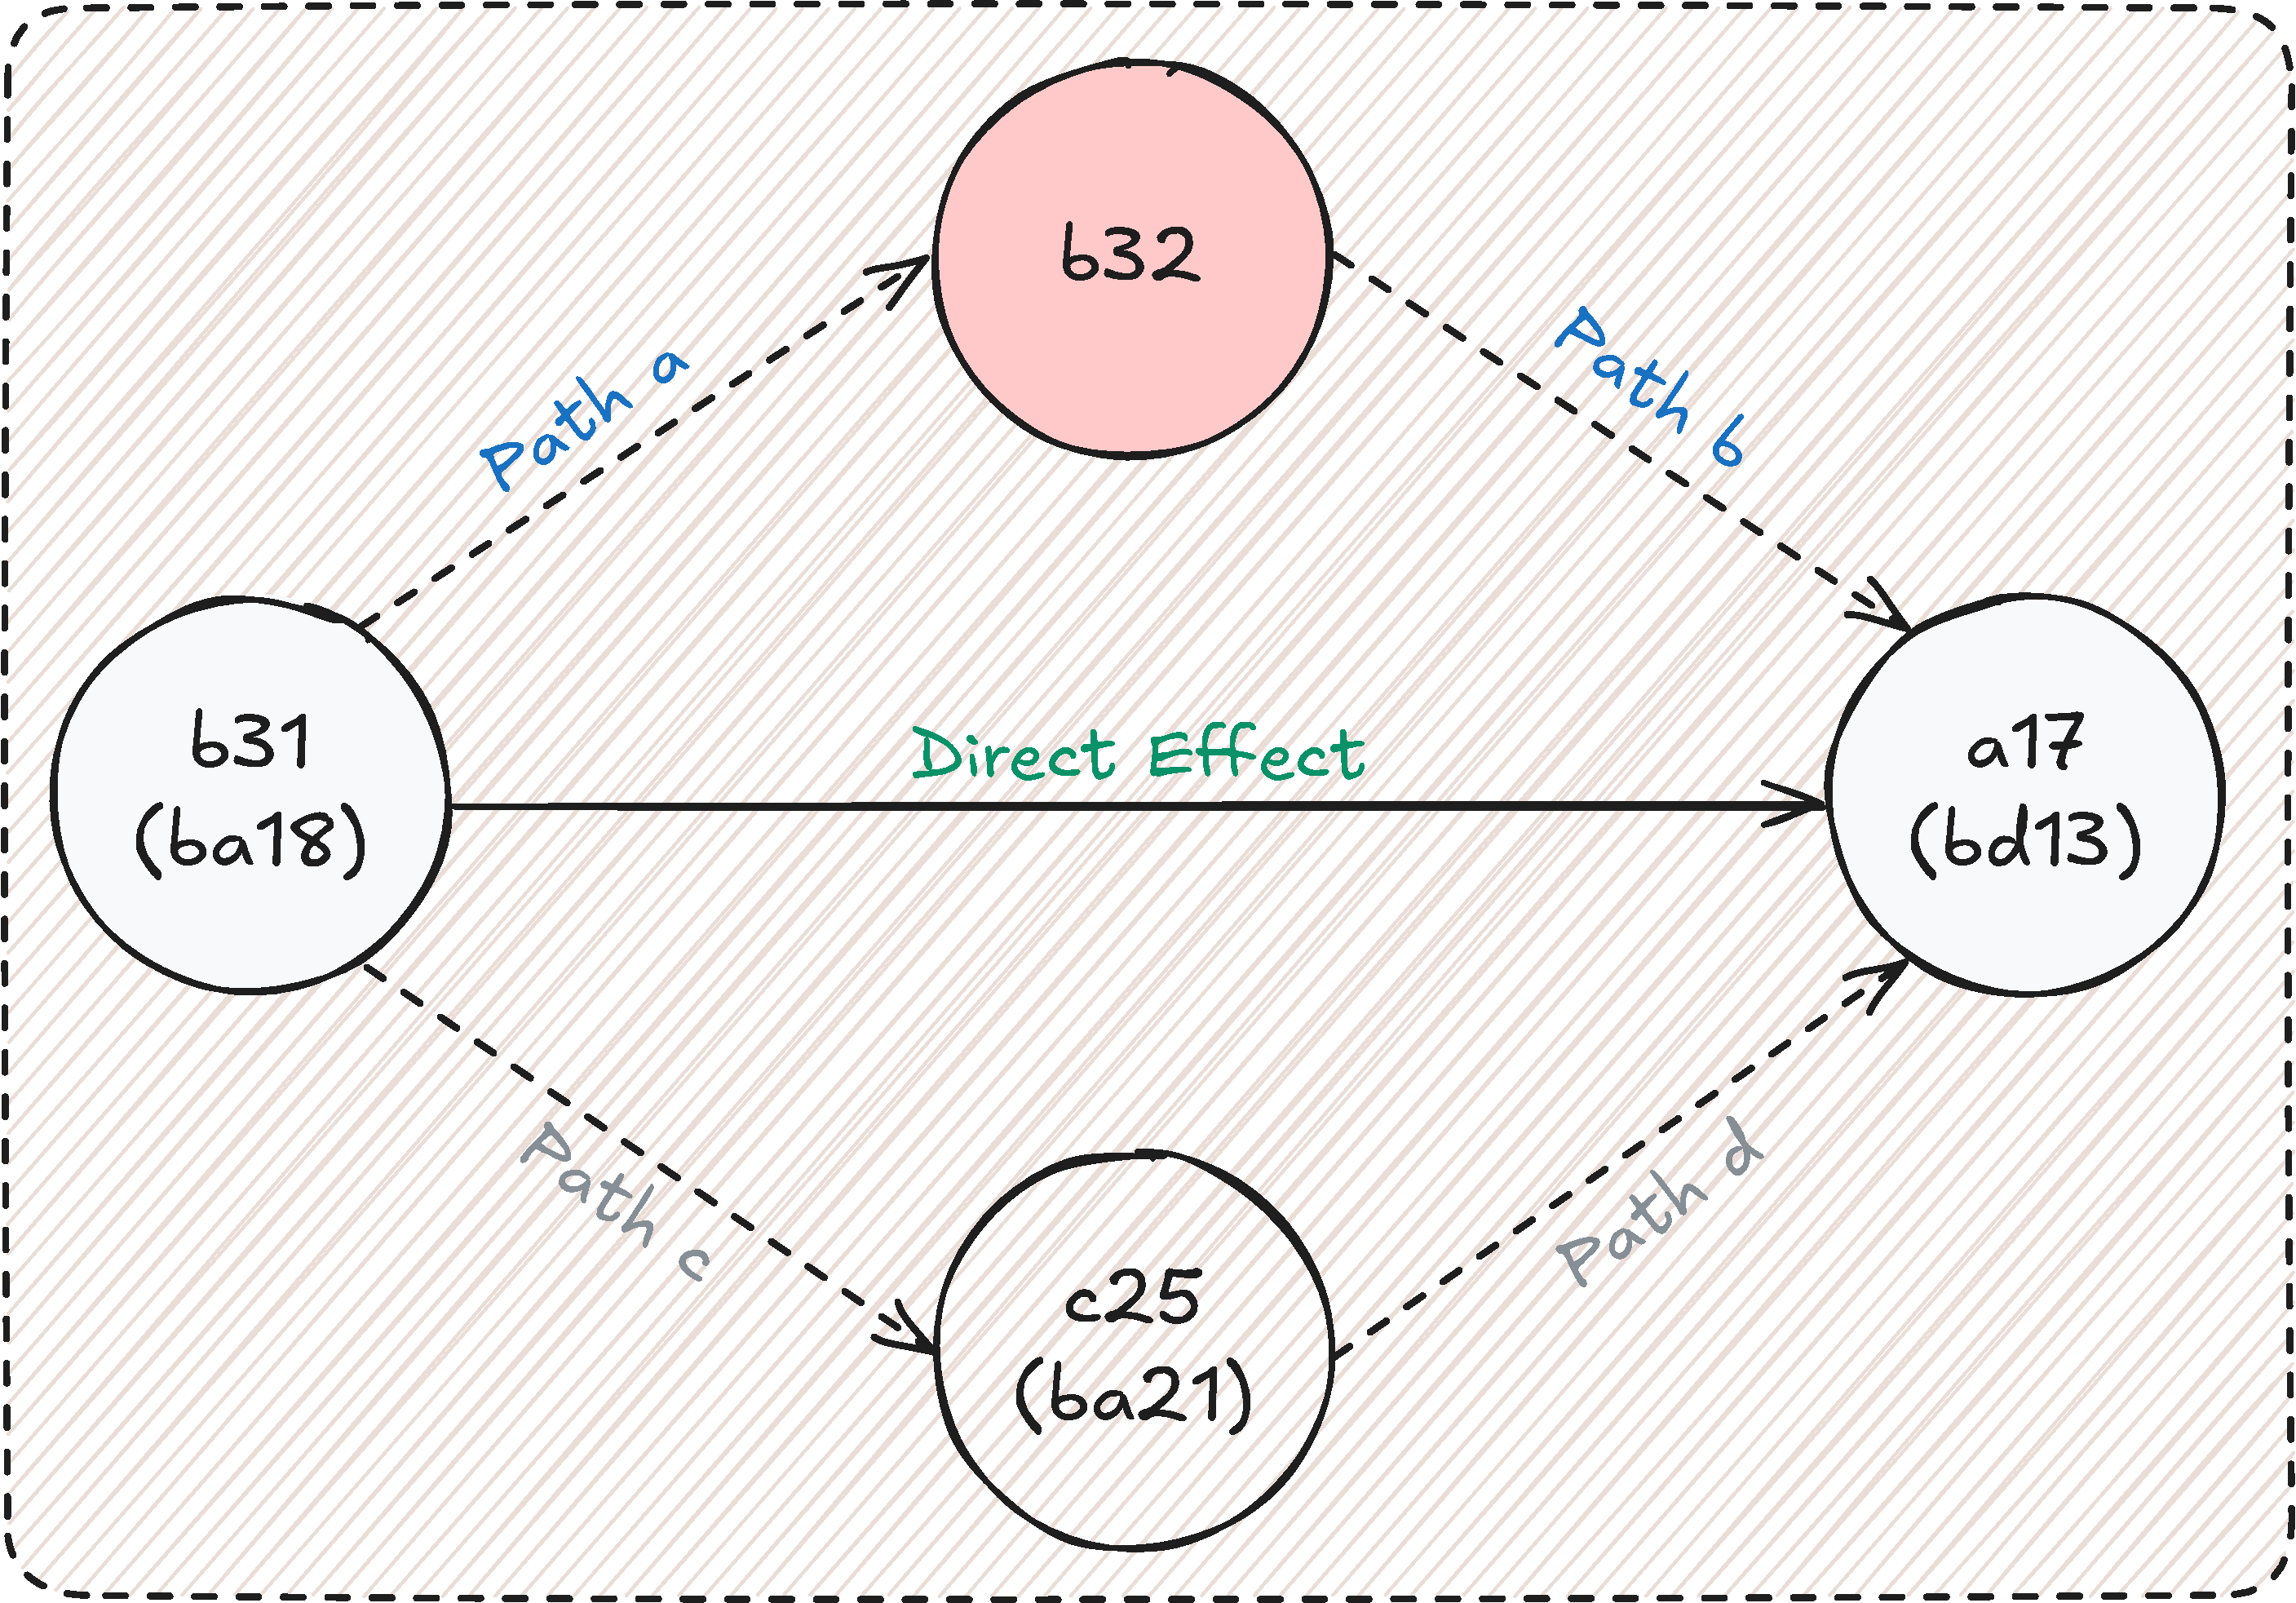
\includegraphics[width=\linewidth]{./figs/pressure.pdf}
        \caption{学业期望压力中介效应模型}\label{figure-pressure}
    \end{minipage}
    \hfill
    \begin{minipage}{0.48\textwidth}
        \centering
        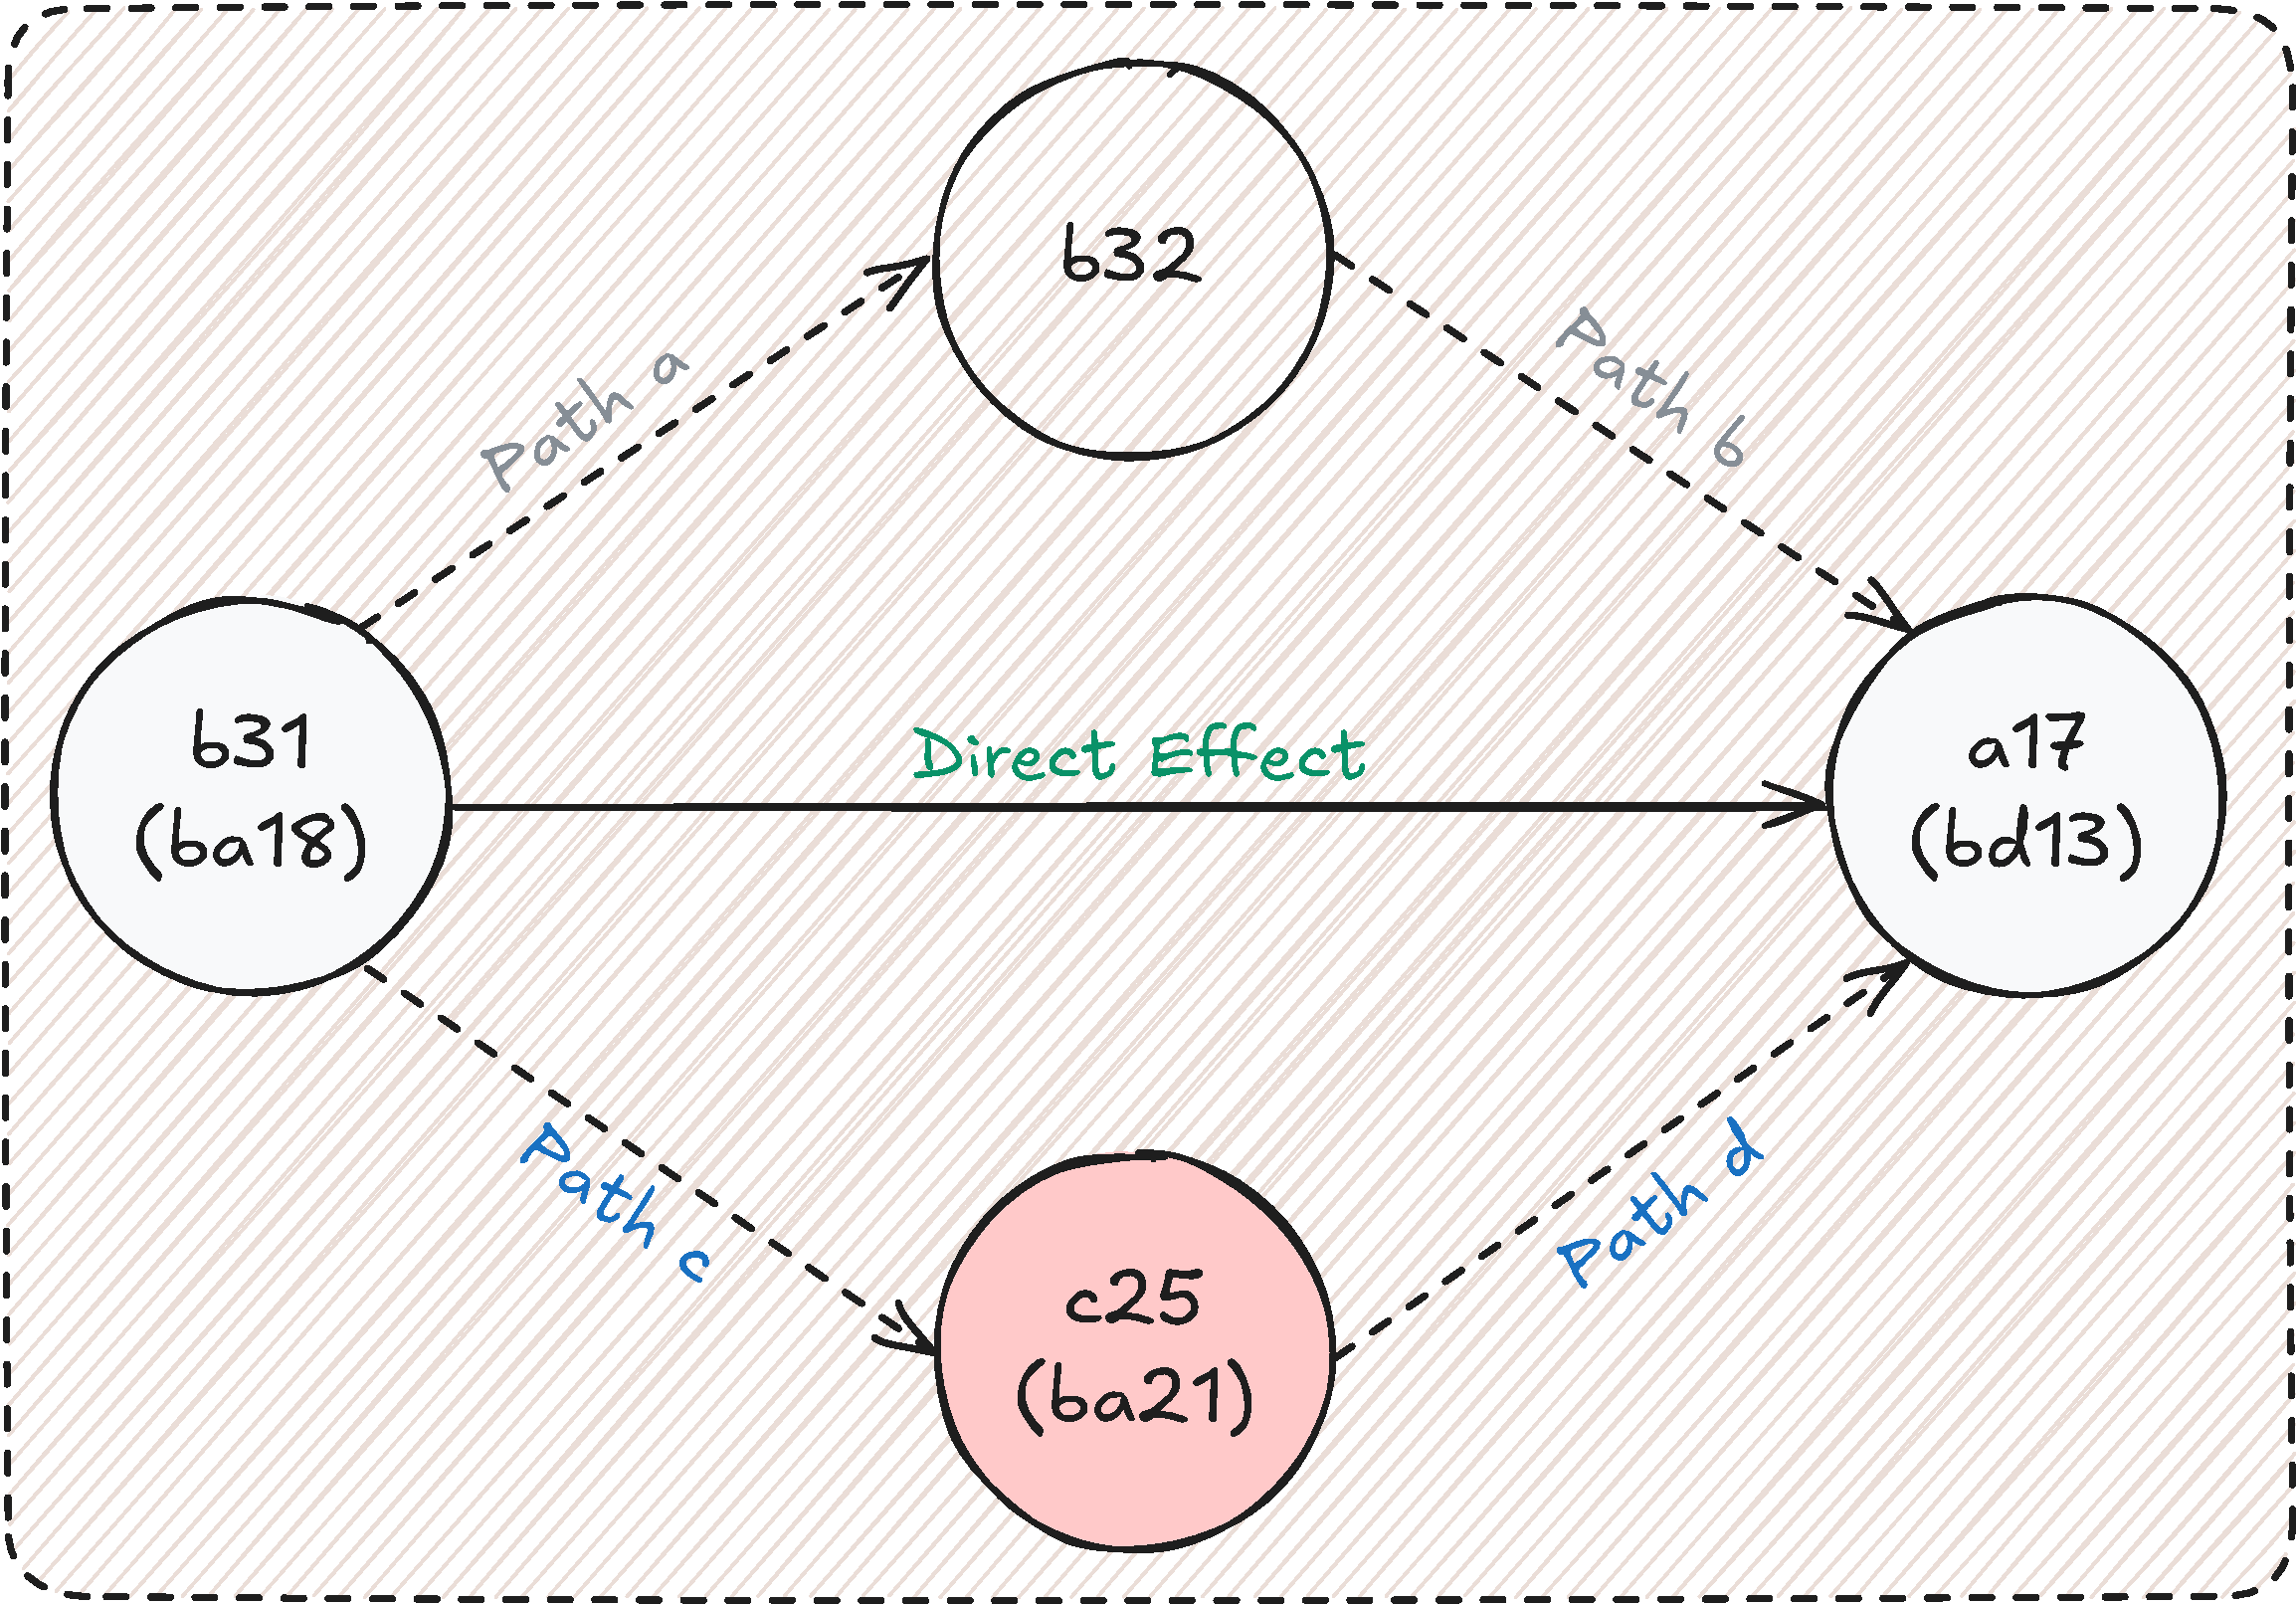
\includegraphics[width=\linewidth]{./figs/confidence.pdf}
        \caption{对未来信心水平中介效应模型}\label{figure-confidence}
    \end{minipage}
\end{figure}

学业压力中介效应模型见图~\ref{figure-pressure} 所示，其中，家庭教育期望直接影响初中生的心理健康，过高的家庭教育期望可能会显著增加青少年学业压力，进而导致心理健康水平下降，产生焦虑、抑郁等负面情绪。在异质性分析中，我们将侧重点放在研究这种家庭教育期望与青少年自身期望的偏差间带来的影响。



\subsubsection{未来信心水平中介变量}
论文将青少年自身对未来的信心水平作为另一个核心的中介变量指标，依然旨在探究外部的家庭期望如何转化为七年级学生个体的内部自我韧性信心水平，并最终影响其心理健康，即对 c25 维度进行测量，数字取值越大表示信心水平越高，具体编号为：

\begin{center}
    \begin{minipage}{1\textwidth}
        \setlength{\columnsep}{0em}
        \setlength{\columnseprule}{0.5pt}
        \begin{multicols}{4}
            \begin{enumerate}
                \item 根本没有信心
                \item 不太有信心
                \item 比较有信心
                \item 很有信心
            \end{enumerate}
        \end{multicols}
    \end{minipage}
\end{center}

信心水平中介效应模型见图~\ref{figure-confidence} 所示，其中，家庭教育期望依然直接影响初中生的心理健康，而过高的家庭教育期望可能会显著减少青少年的信心水平，从而引发心理健康水平降低。在异质性分析中，我们将侧重点放在研究这种家长对孩子信心水平与青少年自身信心程度的偏差间带来的影响。



\subsubsection{控制变量}
我们考虑青少年初中生个体及其家庭背景对心理健康的影响，论文选定学生性别、是否为独生子女、是否有独立的书桌、学生认为家庭经济情况、家长受教育程度、是否领取低保等作为控制变量，旨在探索家庭教育期望对青少年心理健康发展的内隐影响。



\section{研究结果与分析}
\subsection{描述性统计}
七年级的青少年初中生及其家长对教育期望分布见图~\ref{figure-expectation-health} 的教育期望，七年级的青少年初中生及其家长对心理健康分布见图~\ref{figure-expectation-health} 的心理健康，其中，样本总量为 $\bm{6891}$，教育期望中，代码 7 大学本科占据最多，学生希望自己达到大学本科学历约 34.38\%，家长期望子女达到大学本科学历约 37.47\%，心理健康种，代码 5 状态很好占比最多，学生自我心理健康感觉很好约 41.33\%，家长认为青少年子女整体健康很好约 43.94\%。

\begin{figure}[htbp]
    \centering
    \resizebox{\textwidth}{!}{
        \begin{tikzpicture}
            \begin{groupplot}[
                group style = {
                    group size = 2 by 1,
                    horizontal sep = 1cm,
                    vertical sep = 2cm
                },
                ybar = 0pt,
                width = 10cm,
                height = 10cm,
                /pgf/bar width = 9pt,
                ymajorgrids = true,
                grid style = dashed,
                xtick = data,
                enlarge x limits = 0.5,
                tick label style = {font = \scriptsize},
                legend style = {
                    draw = none,
                    font = \footnotesize,
                    anchor = south,
                    /tikz/every even column/.append style = {column sep = 1em}
                },
                legend image code/.code = {
                    \draw [#1, draw = none] (0cm, -0.1cm) rectangle (0.3cm, 0.2cm);
                },
                nodes near coords,
                nodes near coords style = {
                    font = \tiny,
                    color = black,
                    yshift = 1pt,
                    anchor = south,
                    /pgf/number format/fixed,
                    /pgf/number format/precision = 0,
                }
            ]
                \nextgroupplot[
                    ymin = 0,
                    ymax = 2800,
                    symbolic x coords = {b31, ba18},
                    xlabel = {教育期望},
                    legend style = {
                        at = {(0.5, 1.05)},
                        legend columns = 5
                    }
                ]
                \addplot[fill = grad2] coordinates {(b31, 19) (ba18, 7)}; \addlegendentry{1}
                \addplot[fill = grad3] coordinates {(b31, 116) (ba18, 68)}; \addlegendentry{2}
                \addplot[fill = grad4] coordinates {(b31, 166) (ba18, 182)}; \addlegendentry{3}
                \addplot[fill = grad5] coordinates {(b31, 305) (ba18, 180)}; \addlegendentry{4}
                \addplot[fill = grad6] coordinates {(b31, 382) (ba18, 183)}; \addlegendentry{5}
                \addplot[fill = grad7] coordinates {(b31, 1200) (ba18, 841)}; \addlegendentry{6}
                \addplot[fill = grad8] coordinates {(b31, 2369) (ba18, 2582)}; \addlegendentry{7}
                \addplot[fill = grad9] coordinates {(b31, 1099) (ba18, 1311)}; \addlegendentry{8}
                \addplot[fill = grad10] coordinates {(b31, 1036) (ba18, 1537)}; \addlegendentry{9}
                \addplot[fill = grad1] coordinates {(b31, 199) (ba18, 0)}; \addlegendentry{10}

                \nextgroupplot[
                    ymin = 0,
                    ymax = 3300,
                    symbolic x coords = {a17, bd13},
                    xlabel = {心理健康},
                    legend style = {
                        at = {(0.5, 1.05)},
                        legend columns = -1
                    }
                ]
                \addplot[fill = mred1] coordinates {(a17, 40) (bd13, 35)}; \addlegendentry{1}
                \addplot[fill = mred2] coordinates {(a17, 237) (bd13, 168)}; \addlegendentry{2}
                \addplot[fill = mred3] coordinates {(a17, 1425) (bd13, 1319)}; \addlegendentry{3}
                \addplot[fill = mred4] coordinates {(a17, 2341) (bd13, 2341)}; \addlegendentry{4}
                \addplot[fill = mred4] coordinates {(a17, 2848) (bd13, 3028)}; \addlegendentry{5}
            \end{groupplot}
        \end{tikzpicture}
    }
    \vspace*{-2em}
    \caption{青少年教育期望和心理健康与家庭教育期望和心理健康描述统计}\label{figure-expectation-health}
\end{figure}

表~\ref{table-student-statistics} 展示了七年级青少年学生与家长在学业期望一致性上的描述统计结果，通过对多个维度变量交叉分析，可以得出以下结论：

\begin{table}[!t]
    \centering
    \setlength{\tabcolsep}{5pt}
    \renewcommand{\arraystretch}{1}
    \caption{七年级青少年学生的变量描述性统计}\label{table-student-statistics}
    \resizebox{\textwidth}{!}{
        \begin{tabular}{cccccccc}
            \bottomrule[1.5pt]
            \multicolumn{2}{c}{\multirow{2}{*}{\textbf{变量}}} & \multicolumn{2}{c}{$\textbf{家长期望}>\textbf{孩子期望}$} & \multicolumn{2}{c}{$\textbf{家长期望}<\textbf{孩子期望}$} & \multicolumn{2}{c}{$\textbf{家长期望}==\textbf{孩子期望}$} \\
            \cmidrule[0.75pt](lr){3-4} \cmidrule[0.75pt](lr){5-6} \cmidrule[0.75pt](lr){7-8}
            ~ & ~ & \textbf{数量} & \textbf{占比}（\textbf{\%}） & \textbf{数量} & \textbf{占比}（\textbf{\%}） & \textbf{数量} & \textbf{占比}（\textbf{\%}） \\
            \midrule[0.75pt]
            \multirow{2}{*}{性别} & 男 & 1269 & 36.95\% & 698 & 20.33\% & 1467 & 42.72\% \\
            ~ & 女 & 1080 & 31.24\% & 678 & 19.61\% & 1699 & 49.15\% \\
            \addlinespace
            \multirow{2}{*}{独生子} & 是 & 979 & 31.63\% & 618 & 19.97\% & 1498 & 48.40\% \\
            ~ & 否 & 1370 & 36.09\% & 758 & 19.97\% & 1668 & 43.94\% \\
            \addlinespace
            \multirow{2}{*}{独立书桌} & 有 & 1833 & 33.16\% & 1065 & 19.27\% & 2629 & 47.57\% \\
            ~ & 无 & 516 & 37.83\% & 311 & 22.80\% & 537 & 39.37\% \\
            \addlinespace
            \multirow{7}{*}{民族} & 汉 & 2145 & 33.71\% & 1278 & 20.08\% & 2940 & 46.20\% \\
            ~ & 蒙 & 5 & 26.32\% & 7 & 36.84\% & 7 & 36.84\% \\
            ~ & 满 & 32 & 38.55\% & 9 & 10.84\% & 42 & 50.60\% \\
            ~ & 回 & 19 & 34.55\% & 12 & 21.82\% & 24 & 43.64\% \\
            ~ & 藏 & 2 & 28.57\% & 2 & 28.57\% & 3 & 42.86\% \\
            ~ & 壮 & 4 & 80.00\% & 0 & 0.00\% & 1 & 20.00\% \\
            ~ & 其他 & 142 & 39.55\% & 68 & 18.94\% & 149 & 41.50\% \\
            \addlinespace
            \multirow{5}{*}{家长为你做得} & 一点也不多 & 19 & 26.76\% & 23 & 32.39\% & 29 & 40.85\% \\
            ~ & 比较少 & 50 & 33.78\% & 35 & 23.65\% & 63 & 42.57\% \\
            ~ & 不多不少 & 193 & 36.42\% & 122 & 23.02\% & 215 & 40.57\% \\
            ~ & 比较多 & 607 & 37.22\% & 311 & 19.07\% & 713 & 43.72\% \\
            ~ & 非常多 & 1480 & 32.81\% & 885 & 19.62\% & 2146 & 47.57\% \\
            \addlinespace
            \multirow{4}{*}{家长学业成绩要求} & 没有特别要求 & 176 & 35.48\% & 167 & 33.67\% & 153 & 30.85\% \\
            ~ & 班上的平均水平 & 452 & 38.14\% & 235 & 19.83\% & 498 & 42.03\% \\
            ~ & 中上 & 1176 & 36.05\% & 603 & 18.49\% & 1483 & 45.46\% \\
            ~ & 班上前五名 & 545 & 27.98\% & 371 & 19.05\% & 1032 & 52.98\% \\
            \addlinespace
            \multirow{5}{*}{对期望感到} & 毫无压力 & 114 & 30.65\% & 118 & 31.72\% & 140 & 37.63\% \\
            ~ & 有点压力 & 801 & 35.68\% & 368 & 16.39\% & 1076 & 47.93\% \\
            ~ & 一般 & 695 & 37.05\% & 355 & 18.92\% & 826 & 44.03\% \\
            ~ & 压力比较大 & 553 & 32.68\% & 338 & 19.98\% & 801 & 47.34\% \\
            ~ & 压力很大 & 186 & 26.35\% & 197 & 27.90\% & 323 & 45.75\% \\
            \addlinespace
            \multirow{5}{*}{成绩} & 不好 & 203 & 37.80\% & 143 & 26.63\% & 191 & 35.57\% \\
            ~ & 中下 & 506 & 38.36\% & 259 & 19.64\% & 554 & 42.00\% \\
            ~ & 中等 & 702 & 33.85\% & 435 & 20.97\% & 937 & 45.18\% \\
            ~ & 中上 & 759 & 33.35\% & 419 & 18.41\% & 1098 & 48.24\% \\
            ~ & 很好 & 179 & 26.13\% & 120 & 17.52\% & 386 & 56.35\% \\
            \addlinespace
            \multirow{5}{*}{对未来} & 根本没有信心 & 25 & 38.46\% & 21 & 32.31\% & 19 & 29.23\% \\
            ~ & 不太有信心 & 256 & 40.06\% & 130 & 20.34\% & 253 & 39.59\% \\
            ~ & 比较有信心 & 1158 & 36.46\% & 598 & 18.83\% & 1420 & 44.71\% \\
            ~ & 很有信心 & 910 & 30.22\% & 627 & 20.82\% & 1474 & 48.95\% \\
            \toprule[1.5pt]
        \end{tabular}
    }
\end{table}

$\divideontimes$ \textbf{期望一致性的总体分布特征：}在整体样本角度看来，家长期望与青少年孩子期望一致，是当前七年级初中生的主流状态，绝大多数统计变量下，期望一致的学生占比均在 $40\%\sim55\%$ 间，期望不一致的情况下，“家长期望高于孩子期望”显著多于“家长期望低于孩子期望”，这反映了在家庭教育中，家长往往扮演着高标准制定者的角色，而青少年学生自我期望相对有保守务实的倾向。

$\divideontimes$ \textbf{人口学与家庭资源差异特征：}民族方面，由于少数民族样本量极少，不具有代表性，因此我们重点关注汉族，其分布体现的总体趋势是期望一致性 46.20\% 最高，且“家长期望高于孩子期望”比例 33.71\% 显著多于“家长期望低于孩子期望”比例 20.08\%，这反映了汉族家庭中普遍存在“家长主导型”的学业激励模式。性别方面，女生的期望一致性 49.15\% 明显高于男生 42.72\%，而男生中出现“家长期望高于孩子期望”的比例 36.95\% 更高，暗示着家长对男生的学业施压期望偏差可能更大。家庭结构方面，独生子女的期望一致性 48.40\% 更高，非独生子女中家长期望过高的情况更为普遍。我们值得注意的是物质资源也表现出相关性，拥有独立书桌的学生，期望一致性 47.57\% 更高，而没有独立书桌的学生，家长期望高于孩子期望比例 37.83\% 明显上升，隐含出家庭学习环境的缺失可能伴随着沟通成本增加或者教育期望错位。

$\divideontimes$ \textbf{家长投入与学业期望特征：}表~\ref{table-student-statistics} 数据显示，家长的实际投入与教育期望达成共识之间存在可能的正相关关系，随着家长为青少年孩子付出程度的增加，期望一致性的比例从 $40.85\%\to47.57\%$。学业要求上，要求越高，期望一致性的比例反而越高，其中家长要求孩子成绩在“班上前五名”时，期望一致性达到 52.98\% 最高值，而当家长“没有特别要求”时，青少年孩子的自我期望高于家长期望 33.67\% 显著增加，这揭示了明确且高标准的学业目标在某些家庭中已经内化为孩子的自我期望，具备更强的目标共识驱动。

$\divideontimes$ \textbf{压力感受与学业成绩与未来信心表征：}学习成绩越好的学生，其期望与家长期望越容易达成一致，成绩“很好”的学生期望一致性高达 56.35\%，而成绩“不好”的学生中，家长期望过高的比例达到 37.80\%。在心理感受压力层面，感到“中等压力”的学生一致性最强，而处于极端（毫无压力或压力很大）的学生，其期望不一致性比例偏高。在对未来信心水平方面，对未来“很有信心”的学生，其期望一致性 48.95\% 远超过“根本没有信心”的学生 29.23\%，信心不足的青少年中，家长期望远远高于孩子自我期望情况非常突出，有 38.46\% 和 40.06\%，这显现了过高的家长教育期望与青少年学生信心缺失之间可能存在消极联系。

\begin{table}[!t]
    \centering
    \setlength{\tabcolsep}{6pt}
    \renewcommand{\arraystretch}{1}
    \caption{家长的变量描述性统计}\label{table-parent-statistics}
    \begin{threeparttable}
        \resizebox{\textwidth}{!}{
            \begin{tabular}{cccccccc}
                \bottomrule[1.5pt]
                \multicolumn{2}{c}{\multirow{2}{*}{\textbf{变量}}} & \multicolumn{2}{c}{$\textbf{家长期望}>\textbf{孩子期望}$} & \multicolumn{2}{c}{$\textbf{家长期望}<\textbf{孩子期望}$} & \multicolumn{2}{c}{$\textbf{家长期望}==\textbf{孩子期望}$} \\
                \cmidrule[0.75pt](lr){3-4} \cmidrule[0.75pt](lr){5-6} \cmidrule[0.75pt](lr){7-8}
                ~ & ~ & \textbf{数量} & \textbf{占比}（\textbf{\%}） & \textbf{数量} & \textbf{占比}（\textbf{\%}） & \textbf{数量} & \textbf{占比}（\textbf{\%}） \\
                \midrule[0.75pt]
                \multirow{10}{*}{身份} & 生父 & 1007 & 35.43\% & 572 & 20.13\% & 1263 & 44.44\% \\
                ~ & 生母 & 1156 & 32.98\% & 694 & 19.80\% & 1655 & 47.22\% \\
                ~ & 继父 & 3 & 25.00\% & 4 & 33.33\% & 5 & 41.67\% \\
                ~ & 继母 & 2 & 22.22\% & 2 & 22.22\% & 5 & 55.56\% \\
                ~ & （外）祖父 & 76 & 33.04\% & 51 & 22.17\% & 103 & 44.78\% \\
                ~ & （外）祖母 & 42 & 29.37\% & 24 & 16.78\% & 77 & 53.85\% \\
                ~ & 其他男性亲属 & 27 & 54.00\% & 9 & 18.00\% & 14 & 28.00\% \\
                ~ & 其他女性亲属 & 33 & 37.50\% & 16 & 18.18\% & 39 & 44.32\% \\
                ~ & 其他男性非亲属 & 0 & 0.00\% & 1 & 33.33\% & 2 & 66.67\% \\
                ~ & 其他女性非亲属 & 3 & 33.33\% & 3 & 33.33\% & 3 & 33.33\% \\
                \addlinespace
                \multirow{2}{*}{是否报补习班} & 有 & 661 & 31.37\% & 409 & 19.41\% & 1037 & 49.22\% \\
                ~ & 没 & 1688 & 35.28\% & 967 & 20.21\% & 2129 & 44.50\% \\
                \addlinespace
                \multirow{2}{*}{低保} & 是 & 231 & 32.81\% & 158 & 22.44\% & 315 & 44.74\% \\
                ~ & 否 & 2118 & 34.23\% & 1218 & 19.69\% & 2851 & 46.08\% \\
                \addlinespace
                \multirow{5}{*}{家庭经济} & 非常困难 & 107 & 40.68\% & 62 & 23.57\% & 94 & 35.74\% \\
                ~ & 比较困难 & 430 & 37.59\% & 271 & 23.69\% & 443 & 38.72\% \\
                ~ & 中等 & 1709 & 33.51\% & 975 & 19.12\% & 2416 & 47.37\% \\
                ~ & 比较富裕 & 100 & 27.25\% & 62 & 16.89\% & 205 & 55.86\% \\
                ~ & 很富裕 & 3 & 17.65\% & 6 & 35.29\% & 8 & 47.06\% \\
                \addlinespace
                \multirow{4}{*}{对孩子} & 根本没有信心 & 6 & 20.00\% & 13 & 43.33\% & 11 & 36.67\% \\
                ~ & 不太有信心 & 247 & 38.47\% & 162 & 25.23\% & 233 & 36.29\% \\
                ~ & 比较有信心 & 1060 & 32.57\% & 688 & 21.14\% & 1507 & 46.30\% \\
                ~ & 很有信心 & 1036 & 34.95\% & 513 & 17.31\% & 1415 & 47.74\% \\
                \addlinespace
                \multirow{2}{*}{民族} & 汉 & 2169 & 33.81\% & 1291 & 20.12\% & 2955 & 46.06\% \\
                ~ & \cellcolor{MorandiBlue!20}少数民族 & \cellcolor{MorandiBlue!20}180 & \cellcolor{MorandiBlue!20}37.82\% & \cellcolor{MorandiBlue!20}85 & \cellcolor{MorandiBlue!20}17.86\% & \cellcolor{MorandiBlue!20}211 & \cellcolor{MorandiBlue!20}44.33\% \\
                \addlinespace
                \multirow{9}{*}{学历} & 没受过任何教育 & 29 & 27.88\% & 24 & 23.08\% & 51 & 49.04\% \\
                ~ & 小学 & 328 & 36.90\% & 175 & 19.69\% & 386 & 43.42\% \\
                ~ & 初中 & 1026 & 35.45\% & 588 & 20.32\% & 1280 & 44.23\% \\
                ~ & 中专或技校 & 166 & 34.30\% & 88 & 18.18\% & 230 & 47.52\% \\
                ~ & 职业高中 & 101 & 35.07\% & 65 & 22.57\% & 122 & 42.36\% \\
                ~ & 高中 & 261 & 30.46\% & 153 & 17.85\% & 443 & 51.69\% \\
                ~ & 大学专科 & 219 & 31.33\% & 140 & 20.03\% & 340 & 48.64\% \\
                ~ & 大学本科 & 198 & 31.83\% & 131 & 21.06\% & 293 & 47.11\% \\
                ~ & 研究生及以上 & 21 & 38.89\% & 12 & 22.22\% & 21 & 38.89\% \\
                \toprule[1.5pt]
            \end{tabular}
        }
        \begin{tablenotes}\small
            \item 【注】由于少数民族占比量极少，所以用矩形 \cube{MorandiBlue} 归并少数民族结果
        \end{tablenotes}
    \end{threeparttable}
\end{table}

表~\ref{table-parent-statistics} 展示了家长特征在学业期望一致性上的描述统计结果，通过对多个维度变量交叉分析，可以得出以下结论：

$\divideontimes$ \textbf{家庭角色与身份的期望差异：}在家庭核心成员中，生母与孩子的学业期望一致性 47.22\% 略高于生父 44.44\%，期望不一致的情况下，生父表现出更高的“期望高于青少年孩子”的倾向 35.43\%，一个有趣的现象是，（外）祖父母辈在期望一致性上表现突出，尤其是（外）祖母，其一致性比例高达 53.85\%，这可能反映了隔代养育中家长心态相对更平和些，更容易与孩子的自我预期达成共识。

$\divideontimes$ \textbf{补习行为与家庭经济地位的影响：}家长给孩子参报辅导班程度与家庭教育期望一致性呈正相关，报了辅导班的家庭，其学业期望一致性 49.22\% 明显高于未报辅导班的家庭 44.50\%，而未报辅导班家庭中，家长期望过高的比例更高，达到 35.28\%。在经济维度上，家庭经济状况越好，期望一致性越高，从经济“非常困难” 35.74\% 的一致性，逐渐上升至“比较富裕”家庭的 55.86\%，这说明经济资源充裕，可能缓解了家庭内部的学业焦虑，有益于家长在孩子在目标设定上达成对齐。

$\divideontimes$ \textbf{家长信心对期望对齐的心理调节：}家长对青少年孩子的信心程度直接影响了双方期望的吻合度，表~\ref{table-parent-statistics} 数据清晰地显示，随着家长信心的增加，期望一致性比例随之上升，从“根本没有信心”时的 36.67\% 提高至“很有信心”时的 47.74\%。然而，值得警惕的是，当家长“根本没有信心”时，出现了显著的期望倒挂现象，即 43.33\% 的青少年初中生自我期望实际上高于家长期望，这反映了在这类家庭中，孩子可能在缺乏家长支持的情况下，能独自维持极高的学业抱负。

$\divideontimes$ \textbf{学历背景与代际期望偏好：}家长学历对青少年初中生的学业期望影响呈现出复杂性的特征，高中学历家长的期望一致性最高，达到 51.69\%，然而在高学历群体中，譬如研究生及以上，“家长期望高于孩子期望”的比例明显回升，达到 38.89\%，与该群体的一致性比例持平，这可能暗示了高学历家长对孩子拥有更强的代际成就期待，容易给孩子施加超出其自我预期的学业压力。

$\divideontimes$ \textbf{民族分布上差异：}由于少数民族比例很少，因此我们将所有的少数民族样本全部合并，结果表明，汉族维持了 46.06\% 的平均一致性水平，构成整体样本的基准线，而少数民族相对较小。在不一致的情况中，“家长期望高于孩子期望”的比例 33.81\% 显著高于“家长期望低于孩子期望”的 20.12\% 比例，反映出汉族家庭中家长对学业目标设定普遍更具前瞻性和施压性。

$\divideontimes$ \textbf{家庭经济状态特征：}家庭经济状况对家长和孩子的学业期望一致性具有显著塑造作用，总体而言，家庭经济条件的改善与期望达成共识的比例呈现出明显的正相关趋势。在期望一致性方面，随着家庭经济层级提升，家长和青少年初中生达成期望共识比例稳步上升，在“非常困难”的家庭中，期望一致比例最低，仅 35.74\%，而到了“比较富裕”水平时，这一比例显著提升至 55.86\%，成为所有经济组别中的峰值，反映出经济资源充裕往往伴随着更稳定的家庭支持系统和更顺畅的亲子沟通，从而使得双方在学业目标设定上更容易趋于对齐，塑造更健康的青少年心理健康。与此同时，家长的“高期望压力”在经济地位较低的家庭中表现得尤为突出，表~\ref{table-parent-statistics} 数据显示，在“比较困难”和“非常困难”的家庭中，“家长期望高于孩子期望”比例分别高达 40.68\% 和 37.59\%，远高于“比较富裕”家庭的 27.25\%，这代表一种我国社会现象，经济处境差的家长可能更倾向于寄希望于孩子学业成绩优异，从而改变家庭命运，实现社会阶层跃迁的关键路径，因此更容易赋予孩子超出其自我预期的学业压力，从而产生心理不健康等负面情绪。值得注意的是，“很富裕”家庭虽然样本量较小，但呈现出独特的动态特征，该群体中“家长期望低于孩子期望”的比例徒增至 35.29\%，不仅是所有经济层面的最大值，甚至远超该组内“家长期望高于孩子期望”的比例 17.65\%，这可能意味着物质极度优渥的家庭环境中，家长的教育心态转趋平和随意，而青少年孩子受优越环境和资源的影响，其自我实现的驱动力和学业抱负反而可能超过家长的期望要求。此外，在领取低保角度，非低保家庭的期望一致性 46.08\% 略高于低保家庭 44.74\%，进一步印证了经济压力缓解对促进代际学业共识的积极意义。



\subsection{差异性检验}
为探究不同维度对青少年七年级初中生的家庭教育期望和心理健康影响，课程论文采用独立样本 $t$ 检验和多分类变量单因素方差分析。



\subsubsection{独立样本 $t$ 检验}
由于样本量近乎 7000，因此根据中心极限定理~\citep{Moivre,Polya}，我们可以忽略正态性检验。独立样本 $t$ 检验有两种类别，如果方差齐性，则进行 Student 检验，如果方差非齐性，则进行 Welch 检验。因此需要先通过 Levene $F$ 检验，判断两个总体的方差齐性。具体而言，对于 Student 检验，假设两个样本来自的总体方差相等，即 $\sigma_1^2=\sigma_2^2=\sigma^2$，再使用两者的合并方差：
\[ s_{\text{pooled}}^2=\dfrac{\displaystyle(n_1-1)s_1^2+(n_2-1)s_2^2}{n_1+n_2-2} \]

Student 检验的自由度 $df=n_1+n_2-2$，其 $t$ 统计量：
\[ t=\dfrac{\barline{x}_1-\barline{x}_2}{\displaystyle s_{\text{pooled}}^2\sqrt{\dfrac{1}{n_1}+\dfrac{1}{n_2}}} \]

当 $\sigma_1^2\neq\sigma_2^2$，使用 Welch 检验，它使用了修正的等效自由度：
\[ df=\dfrac{\left(\dfrac{\displaystyle s_1^2}{n_1}+\dfrac{\displaystyle s_2^2}{n_2}\right)^2}{\dfrac{1}{n_1-1}\left(\dfrac{\displaystyle s_1^2}{n_1}\right)^2+\dfrac{1}{n_2-1}\left(\dfrac{\displaystyle s_2^2}{n_2}\right)^2} \]

$t$ 分布的概率密度函数 PDF：
\[ f(t,df)=\dfrac{\Gamma\left(\dfrac{df+1}{2}\right)}{\displaystyle\sqrt{df\pi}\cdot\Gamma\left(\dfrac{df}{2}\right)}\left(1+\dfrac{t^2}{df}\right)^{\displaystyle-\dfrac{df+1}{2}} \]

当我们计算显著性水平时，需要涉及 $p$ 值，对于双侧检验：
\[ P=2\int_{|t|}^{\infty}f(s,df)\d s \]

通过不完全 $\beta$ 函数求解 $t$ 统计量对应的 $p$ 值：
\[ \bm{\beta}(x;a,b)=\int_{0}^{x}s^{a-1}(1-s)^{b-1}\d s \]

最终得到：
\[ p=\bm{I}_x(a,b)=\dfrac{\bm{\beta}(x;a,b)}{\bm{\beta}(a,b)} \]

根据这一统计学数学原理，我们编写 C99~\footnote{\href{https://github.com/Illusionna/tiny-stats/blob/main/auto_ttest.c}{https://github.com/Illusionna/tiny-stats/blob/main/auto\_ttest.c}} 语言程序，进行\textbf{全自动化独立样本} $\bm{t}$ \textbf{检验}，终端输出结果如下：

\begin{lstlisting}[
    basicstyle = \ttfamily,
    columns = flexible,
    breaklines = true,
    escapeinside = {!@}{@!}
]
>>> variable: a01 - a17 | alpha = 0.050000
>>> levene_f = 0.647019317596 -> levene_p = 0.421208128168
>>> Student's t-test (homogeneity of variance)
>>> class           count           mean            variance       
>>> 女              3457            4.095169        0.783475       
>>> 男              3434            4.145603        0.806641       
>>> mean_difference =    -0.050434
>>> pooled_var =         0.795019
>>> degree_freedom =     6889.000000
>>> t_value =            -2.347684
>>> p_value =            0.018918686087
>>> Cohen's d =          -0.056563
>>> 95% CI =       (-0.092545 ~ -0.008322)
\end{lstlisting}


为比较青少年学生性别和心理健康两组相互独立的样本，其均值是否存在显著差异，我们进行独立样本 $t$ 检验，表~\ref{table-t-test-gender-health} 所示的是检验结果。

\begin{table}[htbp]
    \centering
    \setlength{\tabcolsep}{5pt}
    \renewcommand{\arraystretch}{1.5}
    \caption{学生性别与心理健康的独立性样本 $t$ 检验结果}\label{table-t-test-gender-health}
    \begin{threeparttable}
        \resizebox{\textwidth}{!}{
            \begin{tabular}{ccccccccccc}
                \bottomrule[1.5pt]
                \textbf{变量} & \textbf{类别} & \textbf{数量} & $\mu\pm\sigma$ & \textbf{均差} & $\displaystyle\sigma^2_{\text{pooled}}$ & $t$ & $df$ & $p$ & Cohen's $d$ & 95\% CI \\
                \midrule[0.75pt]
                \multirow{2}{*}{a17} & 男（1） & 3434 & $4.146\pm0.898$ & \multirow{2}{*}{$-0.050$} & \multirow{2}{*}{0.795} & \multirow{2}{*}{$-2.348$} & \multirow{2}{*}{6889} & \multirow{2}{*}{$\bm{0.019^{*}}$} & \multirow{2}{*}{$-0.057$} & \multirow{2}{*}{$(-0.093\sim-0.008)$} \\
                ~ & 女（0） & 3457 & $4.095\pm0.885$ \\
                \toprule[1.5pt]
            \end{tabular}
        }
        \begin{tablenotes}\small
            \item 【注】$~^{\bm{*}}p < 0.05$，$\displaystyle\sigma^2_{\text{pooled}}$ 是并合方差，Cohen's $d$ 是均值差异效应，CI 是均值差异的信区间
        \end{tablenotes}
    \end{threeparttable}
\end{table}

青少年学生在心理健康水平 a17 维度存在显著的性别差异（$^{\bm{*}}p=0.019<0.05$），具体而言，男生的心理健康得分（$\mu=4.146,\ \sigma=0.898$）显著高于女生（$\mu=4.095,\ \sigma=0.885$），两者的离散程度波动情况基本一致，平均值差值是 $-0.050$，其 95\% 的置信区间为 $(-0.093,\ -0.008)$，不包含 0 点，因此进一步验证了差异的显著性，然而，从 Cohen's $d$ 效应量指标看来，$-0.057$ 绝对值非常小，表明尽管性别差异在统计学上显著，但其实际效应程度极小，在现实生活中的感知可能并不明显。

为比较青少年学生是否为独生子女和心理健康两组相互独立的样本，其均值是否存在显著差异，我们进行独立样本 $t$ 检验，表~\ref{table-t-test-only-child-health} 所示的是检验结果。

\begin{table}[htbp]
    \centering
    \setlength{\tabcolsep}{5pt}
    \renewcommand{\arraystretch}{1.5}
    \caption{学生是否独生子与心理健康的独立性样本 $t$ 检验结果}\label{table-t-test-only-child-health}
    \resizebox{\textwidth}{!}{
        \begin{tabular}{ccccccccccc}
            \bottomrule[1.5pt]
            \textbf{变量} & \textbf{类别} & \textbf{数量} & $\mu\pm\sigma$ & \textbf{均差} & $\displaystyle\sigma^2_{\text{pooled}}$ & $t$ & $df$ & $p$ & Cohen's $d$ & 95\% CI \\
            \midrule[0.75pt]
            \multirow{2}{*}{a17} & 是（1） & 3095 & $4.187\pm0.876$ & \multirow{2}{*}{0.121} & \multirow{2}{*}{0.792} & \multirow{2}{*}{5.597} & \multirow{2}{*}{6889} & \multirow{2}{*}{$\bm{0.000^{*}}$} & \multirow{2}{*}{0.136} & \multirow{2}{*}{$(0.078\sim0.163)$} \\
            ~ & 不是（0） & 3796 & $4.066\pm0.902$ \\
            \toprule[1.5pt]
        \end{tabular}
    }
\end{table}

青少年学生在心理健康水平 a17 维度存在显著的是否独生子女差异（$^{\bm{*}}p=0.000<0.05$）。具体而言，独生子女学生的心理健康得分（$\mu=4.187,\ \sigma=0.876$）显著高于非独生子女学生（$\mu=4.066,\ \sigma=0.902$），两者的离散程度波动情况基本一致。平均值差值是 0.121，其 95\% 的置信区间为 $(0.078,\ 0.163)$，不包含 0 点，因此进一步验证了差异的显著性。从 Cohen's $d$ 效应量指标看来，0.136 表明不仅是否独生子女差异在统计学上显著，而且有一定的实际效应程度。

为比较青少年学生是否有独立的书桌和心理健康两组相互独立的样本，其均值是否存在显著差异，我们进行独立样本 $t$ 检验，表~\ref{table-t-test-desktop-health} 所示的是检验结果。

\begin{table}[htbp]
    \centering
    \setlength{\tabcolsep}{5pt}
    \renewcommand{\arraystretch}{1.5}
    \caption{学生是否有独立的书桌与心理健康的独立性样本 $t$ 检验结果}\label{table-t-test-desktop-health}
    \resizebox{\textwidth}{!}{
        \begin{tabular}{ccccccccccc}
            \bottomrule[1.5pt]
            \textbf{变量} & \textbf{类别} & \textbf{数量} & $\mu\pm\sigma$ & \textbf{均差} & $\displaystyle\sigma^2_{\text{pooled}}$ & $t$ & $df$ & $p$ & Cohen's $d$ & 95\% CI \\
            \midrule[0.75pt]
            \multirow{2}{*}{a17} & 有（1） & 5527 & $4.176\pm0.877$ & \multirow{2}{*}{0.283} & \multirow{2}{*}{0.783} & \multirow{2}{*}{10.596} & \multirow{2}{*}{6889} & \multirow{2}{*}{$\bm{0.000^{*}}$} & \multirow{2}{*}{0.320} & \multirow{2}{*}{$(0.231\sim0.336)$} \\
            ~ & 无（0） & 1364 & $3.893\pm0.915$ \\
            \toprule[1.5pt]
        \end{tabular}
    }
\end{table}

这里有趣的是我们探究了是否有独立书桌对青少年初中生心理健康的影响，通过 $t$ 检验，发现存在极其显著的差异（$^{\bm{*}}p=0.000<0.05$），有独立书桌的学生心理健康得分（$\mu=4.176,\ \sigma=0.877$）显著高于无独立书桌的初中生（$\mu=3.893,\ \sigma=0.915$），两者的离散程度波动情况基本一致。平均值差值是 0.283，其 95\% 的置信区间为 $(0.231,\ 0.336)$，不包含 0 点，因此进一步印证了差异显著性，并且 Cohen's $d$ 效应量指标 0.320 比较高，表明实际效应程度较为明显。

为比较家长本学期是否给青少年初中生报辅导班和心理健康两组相互独立的样本，其均值是否存在显著差异，我们进行独立样本 $t$ 检验，表~\ref{table-t-test-tutoring-health} 所示的是检验结果。

\begin{table}[htbp]
    \centering
    \setlength{\tabcolsep}{5pt}
    \renewcommand{\arraystretch}{1.5}
    \caption{学生是否报名辅导班与心理健康的独立性样本 $t$ 检验结果}\label{table-t-test-tutoring-health}
    \resizebox{\textwidth}{!}{
        \begin{tabular}{ccccccccccc}
            \bottomrule[1.5pt]
            \textbf{变量} & \textbf{类别} & \textbf{数量} & $\mu\pm\sigma$ & \textbf{均差} & $\displaystyle\sigma^2_{\text{pooled}}$ & $t$ & $df$ & $p$ & Cohen's $d$ & 95\% CI \\
            \midrule[0.75pt]
            \multirow{2}{*}{a17} & 有（1） & 2107 & $4.213\pm0.871$ & \multirow{2}{*}{0.134} & \multirow{2}{*}{0.792} & \multirow{2}{*}{5.745} & \multirow{2}{*}{6889} & \multirow{2}{*}{$\bm{0.000^{*}}$} & \multirow{2}{*}{0.150} & \multirow{2}{*}{$(0.088\sim0.179)$} \\
            ~ & 无（0） & 4784 & $4.079\pm0.898$ \\
            \toprule[1.5pt]
        \end{tabular}
    }
\end{table}

青少年初中生在心理健康维度存在显著的是否报名辅导班差异（$^{\bm{*}}p=0.000<0.05$），具体来说，报名辅导班的初中生心理健康得分（$\mu=4.213,\ \sigma=0.871$）显著高于无报名辅导班的学生（$\mu=4.079,\ \sigma=0.898$），两者离散程度波动基本一致，均值差值为 0.134，其 95\% 的置信度区间为 $(0.088,\ 0.179)$，没涉及 0 点，说明差异显著，此外 Cohen's $d$ 效应量指标是 0.150 接近 0.2，表明具备一定的实际效应程度。

为探究家庭是否领取低保和青少年心理健康两组相互独立的样本，其均值是否存在显著差异，我们进行独立样本 $t$ 检验，表~\ref{table-t-test-allowance-health} 所示的是检验结果。

\begin{table}[htbp]
    \centering
    \setlength{\tabcolsep}{5pt}
    \renewcommand{\arraystretch}{1.5}
    \caption{家庭是否领取低保与青少年心理健康的独立性样本 $t$ 检验结果}\label{table-t-test-allowance-health}
    \resizebox{\textwidth}{!}{
        \begin{tabular}{ccccccccccc}
            \bottomrule[1.5pt]
            \textbf{变量} & \textbf{类别} & \textbf{数量} & $\mu\pm\sigma$ & \textbf{均差} & $\displaystyle\sigma^2_{\text{pooled}}$ & $t$ & $df$ & $p$ & Cohen's $d$ & 95\% CI \\
            \midrule[0.75pt]
            \multirow{2}{*}{a17} & 是（1） & 704 & $3.915\pm0.925$ & \multirow{2}{*}{0.229} & \multirow{2}{*}{0.791} & \multirow{2}{*}{6.472} & \multirow{2}{*}{6889} & \multirow{2}{*}{$\bm{0.000^{*}}$} & \multirow{2}{*}{0.257} & \multirow{2}{*}{$(0.160\sim0.298)$} \\
            ~ & 否（0） & 6187 & $4.144\pm0.885$ \\
            \toprule[1.5pt]
        \end{tabular}
    }
\end{table}

青少年七年级学生在家庭是否领取低保方面与其心理健康存在显著差异（$^{\bm{*}}p=0.000<0.05$），家庭没有领取低保的孩子心理健康（$\mu=4.144,\ \sigma=0.885$）显著高于家庭领取低保的孩子心理健康（$\mu=3.915,\ \sigma=0.925$），两者离散程度波动基本一致，均值差异是 0.229，其 95\% 的置信度区间为 $(0.160,\ 0.298)$，不包含 0 点，差异显著，并且 Cohen's $d$ 效应量指标是 0.257，表明实际效应程度较强。



\subsubsection{单因素方差分析}
多于多分类变量，本文采用单因素方差分析，通过比较组间与组内的方差，检验不同水平下，是否对因变量的均值产生显著影响，我们构建的模型检验步骤见图~\ref{figure-ANOVA} 所示。

\begin{figure}[htbp]
    \centering
    \includegraphics*[scale=0.25]{./figs/ANOVA.pdf}
    \caption{多分类变量检验步骤}\label{figure-ANOVA}
\end{figure}

\begin{itemize}
    \item \textbf{Normality 检验：}用于判断样本数据是否来自于正态分布的总体，是决定选择参数检验还是非参数检验的前提，通常 $p\geqslant0.05$ 则表示数据符合正态分布，由于样本量极大，因此中心极限定理保证了均值的正态性~\citep{Moivre,Polya}，所以可以进行图~\ref{figure-ANOVA} 的右分枝检验。
    \item \textbf{Kruskal-Wallis 检验：}通过非参数检验方法比较三个及以上的独立样本组分布是否存在显著差异。
    \item \textbf{Levene 检验：}用于判别多个组别之间的方差是否相等，如果 $p\geqslant0.05$ 方差齐性，则使用标准 ANOVA 参数检验，否则 $p<0.05$ 方差非齐性，则使用 Welch ANOVA 参数检验。
    \item \textbf{ANOVA 检验：}用于比较三个及以上的独立样本组的均值是否存在显著差异，如果 $p<0.05$ 则说明至少有两组之间存在差异。
    \item \textbf{Mann-Whitney U 事后检验：}非参数两两比较，通过两组数据的秩次来确定差异，论文使用 Bonferroni 校正 $p$ 值。
    \item \textbf{Games-Howell 事后检验：}对于 Welch ANOVA 检验结果，依然通过两两比较，对方差非齐性和样本量不平衡的情况具有很强的稳健性。
    \item \textbf{Tukey HSD 事后检验：}对于标准 ANOVA 检验结果，能够严格控制整体类型 $\mathrm{I}$ 错误率，精确找出哪些组别之间存在显著的均值差异。
\end{itemize}

编写模型步骤程序，进行全自动化单因素方差分析，输出结果如下：

\paragraph*{a) b09 家庭经济条件与青少年心理健康}~{}

表~\ref{table-anova-economy-health} 结果显示，Levene 检验显著（$W=11.50,\ p<0.05$），表明组间方差不齐。因此，本研究采用稳健性更强的 Welch's ANOVA 进行均值差异检验。不同家庭经济条件的青少年在心理健康水平上存在显著差异（$F=54.61,\ p<0.05$），效应量偏相关（$\eta^2_p = 0.03361$）。进一步采用 Games-Howell 检验进行事后比较：

\begin{itemize}
    \item 非常困难家庭（$M=3.45$）孩子心理健康得分显著低于其他所有组别（$p<0.05$）；
    \item 比较困难家庭（$M=3.80$）青少年心理健康得分显著低于中等（$M=4.12$）、比较富裕（$M=4.39$）及很富裕（$M=4.48$）家庭（$p<0.05$）；
    \item 中等家庭青少年心理健康得分显著低于比较富裕和很富裕家庭（$p<0.05$）；
    \item 比较富裕与很富裕家庭青少年在心理健康得分上差异不显著（$p=0.946\geqslant0.05$）。
\end{itemize}

\begin{table}[htbp]
    \centering
    \setlength{\tabcolsep}{8pt}
    \renewcommand{\arraystretch}{1.2}
    \caption{家庭经济条件与青少年初中生心理健康单因素检验结果}\label{table-anova-economy-health}
    \begin{tabular}{ccccccc}
        \bottomrule[1.5pt]
        检验类型 & 统计量 & $df1$ & $df2$ & $p$ & $\eta^2_p$ 效应量 \\
        \midrule[0.75pt]
        \makecell{方差齐性检验 \\ Levene's Test} & $W=11.504563$ & 4 & 6886 & $\bm{0.000^{*}}$ & - \\
        \midrule[0.75pt]
        \makecell{均值差异检验 \\ Welch's ANOVA} & $F=54.608052$ & 4 & 269.899562 & $\bm{0.000^{*}}$ & 0.03361 \\
    \end{tabular}
    \setlength{\tabcolsep}{6pt}
    \renewcommand{\arraystretch}{1.2}
    \begin{tabular}{cccccccccc}
        \bottomrule[1.5pt]
        \multicolumn{2}{c}{b09} & \multirow{2}{*}{mean($A$)} & \multirow{2}{*}{mean($B$)} & \multirow{2}{*}{diff} & \multirow{2}{*}{SE} & \multirow{2}{*}{$t$} & \multirow{2}{*}{$df$} & \multirow{2}{*}{$p$} & \multirow{2}{*}{Hedges' $g$} \\
        \cmidrule[0.75pt](lr){1-2}
        $A$ & $B$ \\
        \midrule[0.75pt]
        1 & 2 & 3.451 & 3.803 & -0.353 & 0.123 & -2.875 & 107.688 & $\bm{0.038^{*}}$ & -0.363 \\
        1 & 3 & 3.451 & 4.123 & -0.673 & 0.118 & -5.710 & 91.961 & $\bm{0.000^{*}}$ & -0.765 \\
        1 & 4 & 3.451 & 4.389 & -0.938 & 0.120 & -7.809 & 99.333 & $\bm{0.000^{*}}$ & -1.130 \\
        1 & 5 & 3.451 & 4.483 & -1.033 & 0.171 & -6.037 & 138.502 & $\bm{0.000^{*}}$ & -0.969 \\
        2 & 3 & 3.803 & 4.123 & -0.320 & 0.038 & -8.419 & 862.052 & $\bm{0.000^{*}}$ & -0.362 \\
        2 & 4 & 3.803 & 4.389 & -0.586 & 0.045 & -13.111 & 1344.375 & $\bm{0.000^{*}}$ & -0.676 \\
        2 & 5 & 3.803 & 4.483 & -0.680 & 0.130 & -5.243 & 69.235 & $\bm{0.000^{*}}$ & -0.714 \\
        3 & 4 & 4.123 & 4.389 & -0.265 & 0.029 & -9.124 & 1325.516 & $\bm{0.000^{*}}$ & -0.307 \\
        3 & 5 & 4.123 & 4.483 & -0.360 & 0.125 & -2.874 & 60.137 & $\bm{0.043^{*}}$ & -0.411 \\
        4 & 5 & 4.389 & 4.483 & -0.095 & 0.127 & -0.742 & 64.403 & 0.946 & -0.117 \\
        \toprule[1.5pt]
    \end{tabular}
\end{table}

青少年初中生心理健康水平随着家庭经济条件的改善呈现整体上升趋势，但当经济达到“比较富裕”水平之后，这种增益趋于收敛。

\paragraph*{b) b29 家长对孩子付出多少与青少年心理健康}~{}

表~\ref{table-anova-effort-health} 结果显示，Levene 检验显著（$W=12.97,\ p<0.05$），表明组间方差不齐。因此，本研究采用稳健性更强的 Welch's ANOVA 进行均值差异检验。家长对孩子付出程度不同条件的青少年在心理健康水平上存在显著差异（$F=34.91,\ p<0.05$），效应量偏相关（$\eta^2_p = 0.02263$）。进一步采用 Games-Howell 检验进行事后比较：

\begin{itemize}
    \item 在青少年七年级学生感受到父母较低的付出水平下，组间差异不显著，组别之间未表现出统计学上的显著差异；
    \item 随着付出程度增加，显著性差异开始显现，不多不少的付出程度（$M=3.86$）显著低于比较多付出程度（$M=4.02,\ p=0.007$）和非常多付出（$M=4.21,\ p=0.000$）组别；
    \item 在高投入区间内，提升依然显著，付出程度比较多的家长组别显著低于付出很多的组别（$p=0.000$），表明家长付出程度从“比较多”提升至“非常多”的时候，青少年心理健康水平仍会进一步提升。
\end{itemize}

\begin{table}[htbp]
    \centering
    \setlength{\tabcolsep}{8pt}
    \renewcommand{\arraystretch}{1.2}
    \caption{家长对孩子付出程度与青少年初中生心理健康单因素检验结果}\label{table-anova-effort-health}
    \begin{tabular}{ccccccc}
        \bottomrule[1.5pt]
        检验类型 & 统计量 & $df1$ & $df2$ & $p$ & $\eta^2_p$ 效应量 \\
        \midrule[0.75pt]
        \makecell{方差齐性检验 \\ Levene's Test} & $W=12.973042$ & 4 & 6886 & $\bm{0.000^{*}}$ & - \\
        \midrule[0.75pt]
        \makecell{均值差异检验 \\ Welch's ANOVA} & $F=34.911944$ & 4 & 352.814084 & $\bm{0.000^{*}}$ & 0.022628 \\
    \end{tabular}
    \setlength{\tabcolsep}{6pt}
    \renewcommand{\arraystretch}{1.2}
    \begin{tabular}{cccccccccc}
        \bottomrule[1.5pt]
        \multicolumn{2}{c}{b29} & \multirow{2}{*}{mean($A$)} & \multirow{2}{*}{mean($B$)} & \multirow{2}{*}{diff} & \multirow{2}{*}{SE} & \multirow{2}{*}{$t$} & \multirow{2}{*}{$df$} & \multirow{2}{*}{$p$} & \multirow{2}{*}{Hedges' $g$} \\
        \cmidrule[0.75pt](lr){1-2}
        $A$ & $B$ \\
        \midrule[0.75pt]
        1 & 2 & 3.521 & 3.811 & -0.290 & 0.152 & -1.905 & 123.763 & 0.320 & -0.286 \\
        1 & 3 & 3.521 & 3.864 & -0.343 & 0.136 & -2.518 & 84.907 & 0.096 & -0.352 \\
        1 & 4 & 3.521 & 4.020 & -0.499 & 0.131 & -3.797 & 73.666 & $\bm{0.003^{*}}$ & -0.584 \\
        1 & 5 & 3.521 & 4.206 & -0.685 & 0.130 & -5.251 & 71.435 & $\bm{0.000^{*}}$ & -0.775 \\
        2 & 3 & 3.811 & 3.864 & -0.053 & 0.089 & -0.596 & 233.625 & 0.976 & -0.056 \\
        2 & 4 & 3.811 & 4.020 & -0.209 & 0.082 & -2.555 & 168.020 & 0.084 & -0.245 \\
        2 & 5 & 3.811 & 4.206 & -0.395 & 0.080 & -4.921 & 155.147 & $\bm{0.000^{*}}$ & -0.448 \\
        3 & 4 & 3.864 & 4.020 & -0.156 & 0.046 & -3.362 & 814.013 & $\bm{0.007^{*}}$ & -0.179 \\
        3 & 5 & 3.864 & 4.206 & -0.342 & 0.043 & -7.863 & 639.246 & $\bm{0.000^{*}}$ & -0.385 \\
        4 & 5 & 4.020 & 4.206 & -0.186 & 0.025 & -7.543 & 3000.687 & $\bm{0.000^{*}}$ & -0.214 \\
        \toprule[1.5pt]
    \end{tabular}
\end{table}

家长付出程度对青少年心理健康具有积极的促进作用，且这种促进作用在付出程度达到中等偏上水平后表现得尤为明显。

\paragraph*{c) b30 家长对初中生学业成绩要求与青少年心理健康}~{}

表~\ref{table-anova-requirement-health} 结果显示，Levene 检验显著（$W=5.78,\ p=0.001$），表明组间方差不齐。因此，本研究采用稳健性更强的 Welch's ANOVA 进行均值差异检验。家长对孩子学业成绩要求不同条件的青少年在心理健康水平上存在显著差异（$F=12.08,\ p<0.05$），效应量偏相关（$\eta^2_p = 0.00576$），表明该因素对心理健康变异的解释力较低。进一步采用 Games-Howell 检验进行事后比较：

\begin{itemize}
    \item 低要求组间无显著差异：家长要求为“没有特别要求”的青少年与要求为“班上平均水平”的七年级学生在心理健康得分上差异不显著（$p=0.587$）；
    \item 高要求组间无显著差异：家长要求为“中上水平”与“班上前五名”的青少年心理健康得分也未表现出显著的统计学差异（$p=0.772$）；
    \item 跨区间差异显著：要求为“中上水平”及“前五名”的青少年，其心理健康得分显著高于“没有特别要求”和“平均水平”的组别（$p=0.000$）。
\end{itemize}

\begin{table}[htbp]
    \centering
    \setlength{\tabcolsep}{8pt}
    \renewcommand{\arraystretch}{1.2}
    \caption{家长对孩子学业成绩要求与青少年初中生心理健康单因素检验结果}\label{table-anova-requirement-health}
    \begin{tabular}{ccccccc}
        \bottomrule[1.5pt]
        检验类型 & 统计量 & $df1$ & $df2$ & $p$ & $\eta^2_p$ 效应量 \\
        \midrule[0.75pt]
        \makecell{方差齐性检验 \\ Levene's Test} & $W=5.782154$ & 3 & 6887 & $\bm{0.001^{*}}$ & - \\
        \midrule[0.75pt]
        \makecell{均值差异检验 \\ Welch's ANOVA} & $F=12.082655$ & 3 & 1835.061166 & $\bm{0.000^{*}}$ & 0.005757 \\
    \end{tabular}
    \setlength{\tabcolsep}{6pt}
    \renewcommand{\arraystretch}{1.2}
    \begin{tabular}{cccccccccc}
        \bottomrule[1.5pt]
        \multicolumn{2}{c}{b30} & \multirow{2}{*}{mean($A$)} & \multirow{2}{*}{mean($B$)} & \multirow{2}{*}{diff} & \multirow{2}{*}{SE} & \multirow{2}{*}{$t$} & \multirow{2}{*}{$df$} & \multirow{2}{*}{$p$} & \multirow{2}{*}{Hedges' $g$} \\
        \cmidrule[0.75pt](lr){1-2}
        $A$ & $B$ \\
        \midrule[0.75pt]
        1 & 2 & 3.960 & 4.024 & -0.065 & 0.051 & -1.263 & 887.262 & 0.587 & -0.069 \\
        1 & 3 & 3.960 & 4.148 & -0.189 & 0.046 & -4.078 & 619.829 & $\bm{0.000^{*}}$ & -0.214 \\
        1 & 4 & 3.960 & 4.172 & -0.213 & 0.048 & -4.425 & 716.688 & $\bm{0.000^{*}}$ & -0.236 \\
        2 & 3 & 4.024 & 4.148 & -0.124 & 0.031 & -4.014 & 1983.500 & $\bm{0.000^{*}}$ & -0.140 \\
        2 & 4 & 4.024 & 4.172 & -0.148 & 0.034 & -4.414 & 2411.468 & $\bm{0.000^{*}}$ & -0.164 \\
        3 & 4 & 4.148 & 4.172 & -0.024 & 0.025 & -0.960 & 4026.704 & 0.772 & -0.028 \\
        \toprule[1.5pt]
    \end{tabular}
\end{table}

家长的学业要求和青少年心理健康并非简单的线性负担关系，某种程度上，明确且较高的学业期待可能与更好的心理健康状态相关，不过这种影响的实际强度较小。

\paragraph*{d) b32 学生对期望感到压力程度与青少年心理健康}~{}

表~\ref{table-anova-pressure-health} 结果显示，Levene 检验显著（$W=6.34,\ p<0.05$），表明组间方差不齐。因此，本研究采用稳健性更强的 Welch's ANOVA 进行均值差异检验。学生对期望感到不同程度的压力对青少年心理健康水平存在显著差异（$F=6.69,\ p<0.05$），效应量偏相关（$\eta^2_p = 0.00415$），表明该因素对心理健康变异的解释力很低，更进一步，我们采用 Games-Howell 检验进行事后比较：

\begin{itemize}
    \item 高压力组的健康水平显著下降，压力程度比较大的青少年其心理健康得分显著低于毫无压力的学生（$p=0.015$）和有点压力的学生（$p=0.001$）以及感到一般的学生（$p=0.038$）；
    \item 极端压力组表现类似，压力程度很大的七年级学生，其心理健康得分显著低于毫无压力（$p=0.015$）和有点压力的（$p=0.008$）学生，但与感到压力一般的组相比差异未达到显著水平（$p=0.799$）；
    \item 低压力区间差异并不显著，感到毫无压力的、一般的、有点压力的组别之间，心理健康得分均无统计学显著差异（$p>0.05$）。
\end{itemize}

\begin{table}[htbp]
    \centering
    \setlength{\tabcolsep}{8pt}
    \renewcommand{\arraystretch}{1.2}
    \caption{学生对期望感到压力程度与青少年初中生心理健康单因素检验结果}\label{table-anova-pressure-health}
    \begin{tabular}{ccccccc}
        \bottomrule[1.5pt]
        检验类型 & 统计量 & $df1$ & $df2$ & $p$ & $\eta^2_p$ 效应量 \\
        \midrule[0.75pt]
        \makecell{方差齐性检验 \\ Levene's Test} & $W=6.33807$ & 4 & 6886 & $\bm{0.000^{*}}$ & - \\
        \midrule[0.75pt]
        \makecell{均值差异检验 \\ Welch's ANOVA} & $F=6.690353$ & 4 & 1799.766183 & $\bm{0.000^{*}}$ & 0.004153 \\
    \end{tabular}
    \setlength{\tabcolsep}{6pt}
    \renewcommand{\arraystretch}{1.2}
    \begin{tabular}{cccccccccc}
        \bottomrule[1.5pt]
        \multicolumn{2}{c}{b32} & \multirow{2}{*}{mean($A$)} & \multirow{2}{*}{mean($B$)} & \multirow{2}{*}{diff} & \multirow{2}{*}{SE} & \multirow{2}{*}{$t$} & \multirow{2}{*}{$df$} & \multirow{2}{*}{$p$} & \multirow{2}{*}{Hedges' $g$} \\
        \cmidrule[0.75pt](lr){1-2}
        $A$ & $B$ \\
        \midrule[0.75pt]
        1 & 2 & 4.223 & 4.138 & 0.086 & 0.053 & 1.622 & 498.941 & 0.484 & 0.098 \\
        1 & 3 & 4.223 & 4.167 & 0.056 & 0.052 & 1.065 & 479.516 & 0.824 & 0.064 \\
        1 & 4 & 4.223 & 4.054 & 0.169 & 0.054 & 3.154 & 532.750 & $\bm{0.015^{*}}$ & 0.185 \\
        1 & 5 & 4.223 & 4.030 & 0.193 & 0.061 & 3.146 & 785.434 & $\bm{0.015^{*}}$ & 0.199 \\
        2 & 3 & 4.138 & 4.167 & -0.030 & 0.027 & -1.115 & 4003.326 & 0.799 & -0.035 \\
        2 & 4 & 4.138 & 4.054 & 0.084 & 0.030 & 2.827 & 3472.764 & $\bm{0.038^{*}}$ & 0.095 \\
        2 & 5 & 4.138 & 4.030 & 0.108 & 0.042 & 2.560 & 1124.619 & 0.079 & 0.121 \\
        3 & 4 & 4.167 & 4.054 & 0.114 & 0.029 & 3.970 & 3540.292 & $\bm{0.001^{*}}$ & 0.129 \\
        3 & 5 & 4.167 & 4.030 & 0.138 & 0.041 & 3.326 & 1064.931 & $\bm{0.008^{*}}$ & 0.154 \\
        4 & 5 & 4.054 & 4.030 & 0.024 & 0.043 & 0.556 & 1226.566 & 0.981 & 0.026 \\
        \toprule[1.5pt]
    \end{tabular}
\end{table}

适度的期望压力对心理健康的影响相对稳定，但当压力感知达到很大或者极大的时候，青少年的心理健康水平会显著下降。

\paragraph*{e) b35 家长对孩子是否有信心与青少年心理健康}~{}

表~\ref{table-anova-pconfidence-health} 结果显示，Levene 检验显著（$W=11.14,\ p<0.05$），表明组间方差不齐，因此，本研究采用更稳健更强的 Welch's ANOVA 进行均值差异检验。家长对孩子未来是否有信心与青少年心理健康水平存在显著差异（$F=77.20,\ p<0.05$），效应量偏相关（$\eta^2_p=0.03503$），表明该因素对心理健康变异的解释力很低，更进一步，我采用 Games-Howell 检验进行事后比较：

\begin{itemize}
    \item 低信心组别差异不显著，家长根本没有信心的青少年与不太有信心（$p=0.830$）以及比较有信心（$p=0.083$）的组别在心理健康得分上未达到统计学的显著差异；
    \item 信心水平越高，心理健康得分越高，家长很有信心的组别（$M=4.31$）显著高于其他所有组别（$p<0.05$），同时，比较有信心的组别（$M=4.05$）也显著高于不太有信心的组别（$p<0.05$）；
    \item 家长对孩子信心缺失的负面关联，当家长处于根本没有信心或不太有信心时，青少年的心理健康得分处于较低水平（$M<3.83$）。
\end{itemize}

\begin{table}[htbp]
    \centering
    \setlength{\tabcolsep}{8pt}
    \renewcommand{\arraystretch}{1.2}
    \caption{家长对孩子是否有信心与青少年初中生心理健康单因素检验结果}\label{table-anova-pconfidence-health}
    \begin{tabular}{ccccccc}
        \bottomrule[1.5pt]
        检验类型 & 统计量 & $df1$ & $df2$ & $p$ & $\eta^2_p$ 效应量 \\
        \midrule[0.75pt]
        \makecell{方差齐性检验 \\ Levene's Test} & $W=11.13743$ & 3 & 6887 & $\bm{0.000^{*}}$ & - \\
        \midrule[0.75pt]
        \makecell{均值差异检验 \\ Welch's ANOVA} & $F=77.203764$ & 3 & 290.10974 & $\bm{0.000^{*}}$ & 0.035033 \\
    \end{tabular}
    \setlength{\tabcolsep}{6pt}
    \renewcommand{\arraystretch}{1.2}
    \begin{tabular}{cccccccccc}
        \bottomrule[1.5pt]
        \multicolumn{2}{c}{b35} & \multirow{2}{*}{mean($A$)} & \multirow{2}{*}{mean($B$)} & \multirow{2}{*}{diff} & \multirow{2}{*}{SE} & \multirow{2}{*}{$t$} & \multirow{2}{*}{$df$} & \multirow{2}{*}{$p$} & \multirow{2}{*}{Hedges' $g$} \\
        \cmidrule[0.75pt](lr){1-2}
        $A$ & $B$ \\
        \midrule[0.75pt]
        1 & 2 & 3.698 & 3.825 & -0.126 & 0.148 & -0.850 & 69.301 & 0.830 & -0.129 \\
        1 & 3 & 3.698 & 4.050 & -0.351 & 0.145 & -2.424 & 63.280 & 0.083 & -0.406 \\
        1 & 4 & 3.698 & 4.312 & -0.614 & 0.145 & -4.227 & 63.726 & $\bm{0.000^{*}}$ & -0.703 \\
        2 & 3 & 3.825 & 4.050 & -0.225 & 0.038 & -6.005 & 1068.239 & $\bm{0.000^{*}}$ & -0.256 \\
        2 & 4 & 3.825 & 4.312 & -0.488 & 0.038 & -12.673 & 1171.792 & $\bm{0.000^{*}}$ & -0.549 \\
        3 & 4 & 4.050 & 4.312 & -0.262 & 0.022 & -11.722 & 5577.079 & $\bm{0.000^{*}}$ & -0.305 \\
        \toprule[1.5pt]
    \end{tabular}
\end{table}

家长对孩子的信心程度是影响青少年心理健康的重要保护因素，随着家长信心的增强，青少年的心理健康水平呈现显著上升趋势，尤其家长的充分信心对孩子心理健康具有明显的积极效应。

\paragraph*{f) c12 目前班级成绩与青少年心理健康}~{}

表~\ref{table-anova-score-health} 结果显示，Levene 检验显著（$W=5.52,\ p<0.05$），表明组间方差不齐，因此，论文采用 Welch's ANOVA 进行均值差异检验。学生目前在班级成绩不同与青少年心理健康水平存在显著差异（$F=11.89,\ p<0.05$），效应量偏相关（$\eta^2_p=0.007113$），表明该因素对心理健康变异的解释力很低，所以更进一步，采用 Games-Howell 检验进行事后比较：

\begin{itemize}
    \item 成绩落后组别间差异不显著，成绩评定为不好的青少年与中下水平的青少年在心理健康得分上无显著差异（$p=0.933$）；
    \item 成绩提升与心理健康的关联，成绩为中等的青少年，其心理健康得分（$M=4.12$）显著高于不好及中下组别（$p<0.05$）；
    \item 中上与优秀组别差别不显著，成绩评定为中上的青少年与很好（$p=0.210$）或中等（$p=0.261$）组别之间均未达到统计学上的显著差异。
\end{itemize}

\begin{table}[htbp]
    \centering
    \setlength{\tabcolsep}{8pt}
    \renewcommand{\arraystretch}{1.2}
    \caption{学生目前班级成绩与青少年初中生心理健康单因素检验结果}\label{table-anova-score-health}
    \begin{tabular}{ccccccc}
        \bottomrule[1.5pt]
        检验类型 & 统计量 & $df1$ & $df2$ & $p$ & $\eta^2_p$ 效应量 \\
        \midrule[0.75pt]
        \makecell{方差齐性检验 \\ Levene's Test} & $W=5.517366$ & 4 & 6886 & $\bm{0.000^{*}}$ & - \\
        \midrule[0.75pt]
        \makecell{均值差异检验 \\ Welch's ANOVA} & $F=11.892171$ & 4 & 2141.842538 & $\bm{0.000^{*}}$ & 0.007113 \\
    \end{tabular}
    \setlength{\tabcolsep}{6pt}
    \renewcommand{\arraystretch}{1.2}
    \begin{tabular}{cccccccccc}
        \bottomrule[1.5pt]
        \multicolumn{2}{c}{c12} & \multirow{2}{*}{mean($A$)} & \multirow{2}{*}{mean($B$)} & \multirow{2}{*}{diff} & \multirow{2}{*}{SE} & \multirow{2}{*}{$t$} & \multirow{2}{*}{$df$} & \multirow{2}{*}{$p$} & \multirow{2}{*}{Hedges' $g$} \\
        \cmidrule[0.75pt](lr){1-2}
        $A$ & $B$ \\
        \midrule[0.75pt]
        1 & 2 & 3.987 & 4.025 & -0.038 & 0.048 & -0.791 & 980.991 & 0.933 & -0.041 \\
        1 & 3 & 3.987 & 4.117 & -0.130 & 0.045 & -2.880 & 804.394 & $\bm{0.033^{*}}$ & -0.144 \\
        1 & 4 & 3.987 & 4.170 & -0.184 & 0.044 & -4.132 & 753.438 & $\bm{0.000^{*}}$ & -0.212 \\
        1 & 5 & 3.987 & 4.251 & -0.264 & 0.053 & -5.008 & 1109.803 & $\bm{0.000^{*}}$ & -0.291 \\
        2 & 3 & 4.025 & 4.117 & -0.092 & 0.032 & -2.855 & 2730.570 & $\bm{0.035^{*}}$ & -0.101 \\
        2 & 4 & 4.025 & 4.170 & -0.145 & 0.031 & -4.669 & 2552.560 & $\bm{0.000^{*}}$ & -0.166 \\
        2 & 5 & 4.025 & 4.251 & -0.226 & 0.042 & -5.360 & 1456.247 & $\bm{0.000^{*}}$ & -0.248 \\
        3 & 4 & 4.117 & 4.170 & -0.053 & 0.027 & -2.010 & 4254.903 & 0.261 & -0.061 \\
        3 & 5 & 4.117 & 4.251 & -0.134 & 0.039 & -3.445 & 1189.602 & $\bm{0.005^{*}}$ & -0.150 \\
        4 & 5 & 4.170 & 4.251 & -0.081 & 0.038 & -2.124 & 1096.365 & 0.210 & -0.094 \\
        \toprule[1.5pt]
    \end{tabular}
\end{table}

学业成绩的优劣与青少年心理健康水平呈现正相关趋势，表现为成绩好的学生心理健康水平相对越高，但这种影响主要体验在“成绩优秀”与“成绩落后”组别的对比中，在中等成绩区间内，这种关联性表现得较为模糊。

\paragraph*{g) c25 自己对未来是否有信心与青少年心理健康}~{}

表~\ref{table-anova-sconfidence-health} 结果显示，Levene 检验显著（$W=8.75,\ p<0.05$），表明组间方差不齐，因此，采用 Welch's ANOVA 进行均值差异检验。学生对自己未来信心水平不同与青少年心理健康水平存在显著差异（$F=82.53,\ p<0.05$），效应量偏相关（$\eta^2_p=0.037378$），表明该因素对心理健康变异的解释力很低，更进一步采用 Games-Howell 检验进行事后：

\begin{itemize}
    \item 低信心区间差异不显著，对自己未来根本没有信心与不太有信心的青少年初中生在心理健康得分上无显著差异（$p=0.556$）；
    \item 信心提升带来的心理更健康显著获益，对自己未来比较有信心（$M=4.03$）的青少年，其心理健康得分显著高于根本没有信心（$M=3.62$）和不太有信心（$M=3.81$）的组别（$p<0.05$）；
    \item 高信心组的领先优势，对自己未来很有信心的青少年（$M=4.30$），其心理健康得分显著高于其他所有信心程度较低的组别（$p=0.000<0.001$）。
\end{itemize}

\begin{table}[htbp]
    \centering
    \setlength{\tabcolsep}{8pt}
    \renewcommand{\arraystretch}{1.2}
    \caption{自己对未来信心程度与青少年初中生心理健康单因素检验结果}\label{table-anova-sconfidence-health}
    \begin{tabular}{ccccccc}
        \bottomrule[1.5pt]
        检验类型 & 统计量 & $df1$ & $df2$ & $p$ & $\eta^2_p$ 效应量 \\
        \midrule[0.75pt]
        \makecell{方差齐性检验 \\ Levene's Test} & $W=8.753575$ & 3 & 6887 & $\bm{0.000^{*}}$ & - \\
        \midrule[0.75pt]
        \makecell{均值差异检验 \\ Welch's ANOVA} & $F=82.529997$ & 3 & 294.591032 & $\bm{0.000^{*}}$ & 0.037378 \\
    \end{tabular}
    \setlength{\tabcolsep}{6pt}
    \renewcommand{\arraystretch}{1.2}
    \begin{tabular}{cccccccccc}
        \bottomrule[1.5pt]
        \multicolumn{2}{c}{c25} & \multirow{2}{*}{mean($A$)} & \multirow{2}{*}{mean($B$)} & \multirow{2}{*}{diff} & \multirow{2}{*}{SE} & \multirow{2}{*}{$t$} & \multirow{2}{*}{$df$} & \multirow{2}{*}{$p$} & \multirow{2}{*}{Hedges' $g$} \\
        \cmidrule[0.75pt](lr){1-2}
        $A$ & $B$ \\
        \midrule[0.75pt]
        1 & 2 & 3.615 & 3.806 & -0.191 & 0.145 & -1.315 & 73.607 & 0.556 & -0.196 \\
        1 & 3 & 3.615 & 4.025 & -0.409 & 0.141 & -2.908 & 65.526 & $\bm{0.025^{*}}$ & -0.473 \\
        1 & 4 & 3.615 & 4.299 & -0.684 & 0.141 & -4.856 & 65.654 & $\bm{0.000^{*}}$ & -0.780 \\
        2 & 3 & 3.806 & 4.025 & -0.219 & 0.041 & -5.375 & 858.350 & $\bm{0.000^{*}}$ & -0.250 \\
        2 & 4 & 3.806 & 4.299 & -0.493 & 0.041 & -12.049 & 877.458 & $\bm{0.000^{*}}$ & -0.557 \\
        3 & 4 & 4.025 & 4.299 & -0.274 & 0.022 & -12.482 & 6157.524 & $\bm{0.000^{*}}$ & -0.318 \\
        \toprule[1.5pt]
    \end{tabular}
\end{table}

综上所述，七年级青少年学生对自己未来的信心程度与其的心理健康水平呈现显著的正相关关系，个体对未来的预期越积极，其心理健康状态越好，而且这种心理层面的自我评价对心理健康的影响强度超过了客观学业成绩或家长要求等外部因素。



\subsection{相关性分析}
结合显著性差异检验，我们探索家庭教育期望、学业压力、未来信心水平等多个因素与青少年心理健康程度之间的线性关系，此处采用 Pearson 相关分析，该公式系数 $r$ 用于衡量两个变量之间的线性相关强度与方向~\citep{Pearson}。
\[ r=\dfrac{\displaystyle\sum_{i=1}^{n}\left(x_i-\barline{x}\right)\left(y_i-\barline{y}\right)}{\sqrt{\displaystyle\sum_{i=1}^{n}\left(x_i-\barline{x}\right)^2}\sqrt{\displaystyle\sum_{i=1}^{n}\left(y_i-\barline{y}\right)^2}}\in[-1,\ 1] \]

表~\ref{table-pearson} 展现了相关性分析结果，图~\ref{figure-pearson} 是根据表~\ref{table-pearson} 数据绘制而来，其中气泡大小代表相关性系数 $r$ 的取值，红色代表正相关，蓝色代表负相关。

\begin{table}[htbp]
    \centering
    \setlength{\tabcolsep}{12pt}
    \renewcommand{\arraystretch}{1.2}
    \caption{Pearson 相关分析结果}\label{table-pearson}
    % \resizebox{\textwidth}{!}{
        \begin{tabular}{ccccccc}
            \bottomrule[1.5pt]
            $A$ & $B$ & $r$ & $p$ & 95\% CI & BF10 & power \\
            \midrule[0.75pt]
            b09 & b29 & 0.018 & 0.138 & $(-0.01\sim0.04)$ & 0.045 & 0.317 \\
            b09 & b30 & 0.029 & 0.014 & $(0.01\sim0.05)$ & 0.302 & 0.687 \\
            b09 & b32 & -0.088 & 0.000 & $(-0.11\sim-0.06)$ & 4.98e+09 & 1.000 \\
            b09 & b35 & 0.142 & 0.000 & $(0.12\sim0.17)$ & 5.033e+28 & 1.000 \\
            b09 & c12 & 0.097 & 0.000 & $(0.07\sim0.12)$ & 2.042e+12 & 1.000 \\
            b09 & c25 & 0.127 & 0.000 & $(0.1\sim0.15)$ & 3.024e+22 & 1.000 \\
            b09 & a17 & 0.181 & 0.000 & $(0.16\sim0.2)$ & 1.297e+48 & 1.000 \\
            b29 & b30 & 0.100 & 0.000 & $(0.08\sim0.12)$ & 1.336e+13 & 1.000 \\
            b29 & b32 & -0.027 & 0.028 & $(-0.05\sim-0.00)$ & 0.17 & 0.595 \\
            b29 & b35 & 0.271 & 0.000 & $(0.25\sim0.29)$ & 4.398e+112 & 1.000 \\
            b29 & c12 & 0.083 & 0.000 & $(0.06\sim0.11)$ & 2.607e+08 & 1.000 \\
            b29 & c25 & 0.190 & 0.000 & $(0.17\sim0.21)$ & 1.344e+53 & 1.000 \\
            b29 & a17 & 0.149 & 0.000 & $(0.13\sim0.17)$ & 6.246e+31 & 1.000 \\
            b30 & b32 & 0.021 & 0.080 & $(-0.00\sim0.04)$ & 0.07 & 0.417 \\
            b30 & b35 & 0.200 & 0.000 & $(0.18\sim0.22)$ & 3.126e+59 & 1.000 \\
            b30 & c12 & 0.476 & 0.000 & $(0.46\sim0.49)$ & $\infty$ & 1.000 \\
            b30 & c25 & 0.177 & 0.000 & $(0.15\sim0.2)$ & 4.392e+45 & 1.000 \\
            b30 & a17 & 0.071 & 0.000 & $(0.05\sim0.09)$ & 4.886e+05 & 1.000 \\
            b32 & b35 & -0.147 & 0.000 & $(-0.17\sim-0.12)$ & 1.108e+31 & 1.000 \\
            b32 & c12 & -0.179 & 0.000 & $(-0.2\sim-0.16)$ & 7.547e+46 & 1.000 \\
            b32 & c25 & -0.160 & 0.000 & $(-0.18\sim-0.14)$ & 7.295e+36 & 1.000 \\
            b32 & a17 & -0.063 & 0.000 & $(-0.09\sim-0.04)$ & 1.275e+04 & 0.999 \\
            b35 & c12 & 0.287 & 0.000 & $(0.26\sim0.31)$ & 2.441e+126 & 1.000 \\
            b35 & c25 & 0.565 & 0.000 & $(0.55\sim0.58)$ & $\infty$ & 1.000 \\
            b35 & a17 & 0.186 & 0.000 & $(0.16\sim0.21)$ & 1.144e+51 & 1.000 \\
            c12 & c25 & 0.264 & 0.000 & $(0.24\sim0.29)$ & 2.067e+106 & 1.000 \\
            c12 & a17 & 0.084 & 0.000 & $(0.06\sim0.11)$ & 4.614e+08 & 1.000 \\
            c25 & a17 & 0.193 & 0.000 & $(0.17\sim0.22)$ & 5.308e+54 & 1.000 \\
            \toprule[1.5pt]
        \end{tabular}
    % }
\end{table}

表~\ref{table-pearson} 和图~\ref{figure-pearson} 的分析结果表明，各变量之间呈现出复杂的关联网络，总体而言，信心维度变量与学业表现之间存在极强的正相关，而学业压力普遍对青少年身心健康及自信心产生显著的负面影响，具体而言有如下结论：

$\divideontimes$ \textbf{信心传递机制与学业表现：}父母对未来的信心与学生对自己未来的信心之间表现出整个数据集中最强的正相关关系（$r=0.565,\ p<0.001$），这表明家庭内部的信心具有极高的传递性，父母的态度直接映射了学生的自我认识。学生目前的班级排名与家长信心（$r=0.287$）及学生自我信心（$r=0.264$）均呈现显著正相关，说明优异的学业表现是建立自信的基础，同时也不仅受限于学生自身，还显著到家长态度的影响。

$\divideontimes$ \textbf{家长期望与学业压力的双面效应：}家长的学业成绩要求与学生实际班级排名呈现极强的正相关（$r=0.476,\ p<0.001$），这意味在数据上体现为，家长要求越高，趋向“班上前五名”，学生的实际排名往往越靠前。对于期望感受到压力与几乎所有积极指标呈现显著负相关，压力越大，学生的自我信心越低（$r=-0.160$），父母信心越低（$r=-0.147$），且目前的班级排名越靠后（$r=-0.179$），提示了单纯的心理压力并不能转化为学业动力，反而与较差的学业表现和低自信心相伴生。

\begin{figure}[htbp]
    \centering
    \includegraphics*[scale=0.75]{./figs/pearson.pdf}
    \caption{变量相关性分析系数矩阵（气泡越大相关性越强）}\label{figure-pearson}
\end{figure}

$\divideontimes$ \textbf{健康状况的多维影响因素：}青少年七年级初中生的现在整体健康情况，分析显示心理资本比物质条件更能预测健康感知。心理因素能起主导作用，自我信心（$r=0.193$）和父母信心（$r=0.186$）是与健康状况正相关性最强的两个变量，这揭示对自己未来的乐观预期与当前的身心健康紧密相连。物质与支持基础，家庭经济条件（$r=0.181$）与家长提供的支持（$r=0.149$）也与健康呈显著正相关，但相关系数略低于信心变量。学业压力与健康状况呈现显著负相关（$r=-0.063,\ p<0.001$），虽然系数绝对值较小，但在统计上确认了压力对健康的损耗作用。

$\divideontimes$ \textbf{家庭背景与教育投入的独立性：}家长为孩子的付出程度与其对孩子未来的信心之间存在中等强度的显著正相关（$r=0.271,\ p<0.001$），说明投入感与积极预期在家庭系统中是并行的。家庭背景与教育投入的独立性，值得注意的是，家庭经济条件与父母为孩子做事情之间不存在显著相关性（$r=0.018,\ p=0.138$），这表明家长对孩子的日常投入和照顾并不受制于家庭的经济富裕程度，不同经济阶层的家长在为孩子做事的程度上没有显著差异。家长的学业要求与学生感受压力之间的相关性未达到显著水平（$r=0.021,\ p=0.080$），暗示压力可能来源于学生对要求的内化程度而非要求本身。



\subsection{多元线性回归}
在控制人口学特征和家庭背景变量后，验证“家庭教育期望”对“七年级青少年初中生心理健康”是否存在显著的直接影响，并确定影响方向和程度，本节渗透回归哲学理念，采用线性回归方法，逐步增加变量，以观察不同变量组对心理健康的解释力度变化。

控制变量的基线回归方程如下：
\[ Y=\lambda_0+\lambda_1C_1+\lambda_2C_2+\ldots+\lambda_mC_m+\varepsilon \]

全模型方程如下：
\[ Y=\lambda_0+\lambda_1C_1+\lambda_2C_2+\ldots+\lambda_mC_m+\bm{\varLambda}\bm{X}^{\top}+\varepsilon \]

通过最小化残差平方和 RSS 求解系数 $\lambda$，即最小二乘法~\citep{Legendre}：
\[ \text{RSS}=\displaystyle\sum_{i=1}^{n}\left(Y_i-\widehat{Y}_i\right)^2=\displaystyle\sum_{i=1}^{n}\left[Y_i-\left(\lambda_0+\sum_{i=1}^{m}\lambda_iC_i+\bm{\varLambda}\bm{X}^{\top}\right)\right]^2 \]

多元线性回归的关键不在于单次回归，而在于模型对比，通过计算两个模型的决定系数之差 $\Delta R^2$，我们可以判断新加入的变量是否对模型贡献显著的额外解释力。表~\ref{table-baseline} 是控制变量 $C$ 的回归结果，包含了学生性别、是否为独生子女、是否有独立的书桌、本学期是否报辅导班、家庭经济条件、是否领取低保。

\begin{table}[htbp]
    \centering
    \setlength{\tabcolsep}{7pt}
    \renewcommand{\arraystretch}{1.2}
    \caption{控制变量基准回归 Baseline 结果}\label{table-baseline}
    % \resizebox{\textwidth}{!}{
        \begin{tabular}{cccccc}
            \bottomrule[1.5pt]
            控制变量 & Coef. & Std. Err. & $p$ & 95\% CI & VIF \\
            \midrule[0.75pt]
            Intercept & 3.6474 & 92.282 & 0.000 & $(3.570\sim3.725)$ & - \\
            a01 & 0.0601 & 2.829 & 0.005 & $(0.018\sim0.102)$ & 1.859402 \\
            b01 & 0.0220 & 0.966 & 0.334 & $(-0.023\sim0.067)$ & 2.087652 \\
            b11 & 0.1879 & 6.546 & 0.000 & $(0.132\sim0.244)$ & 5.218965 \\
            ba0 & 0.0422 & 1.729 & 0.084 & $(-0.006\sim0.090)$ & 1.627338 \\
            be19 & 0.1560 & 8.167 & 0.000 & $(0.119\sim0.193)$ & 5.707449 \\
            be20 & -0.1350 & -3.774 & 0.000 & $(-0.205\sim-0.065)$ & 1.094503 \\
            \midrule[0.75pt]
            \multicolumn{6}{c}{Baseline 回归拟合统计量} \\
            \midrule[0.75pt]
            $df$ & 6884 & $R^2$ & \fcolorbox{MorandiOrange}{white}{\cube{MorandiOrange} 0.032} & Adj. $R^2$ & 0.031 \\
            $F$ & 37.87 & $p$ & 1.77e-45 & RMSE & 0.878 \\
            AIC & 17770 & BIC & 17820 & $\displaystyle\prod\log$ & -8877.4 \\
            Omnibus & 481.246 & Durbin-Watson & 1.907 & Kurtosis & 3.026 \\
            Skew & -0.716 & Jarque-Bera & 588.846 & Cond No. & 10.4 \\
            \toprule[1.5pt]
        \end{tabular}
    % }
\end{table}

我们首先构建了一个基准回归 Baseline 模型，旨在考察一系列控制变量（性别、是否独生子女、家庭经济背景等）对学生整体心理健康情况的影响。从回归拟合统计量来看，模型的 $F$ 统计量（$37.87,\ p<0.001$）表明模型整体具有统计学意义。在共线性检验方面，所有变量的方差膨胀因子 VIF 均处于合理范围内（最大值为 $5.71$），表明模型不存在严重的多重共线性问题，此外，Durbin-Watson 统计量为 $1.907$，说明残差项不存在明显的自相关。回归结果显示，多个控制变量对学生心理健康状况具有显著影响：

\begin{itemize}
    \item \textbf{性别（a01）：} 系数为 $0.0601$（$p < 0.01$），表明在控制其他因素时，男生的心理健康状况显著高于女生；
    \item \textbf{是否有独立的书桌（b11）：} 是否拥有独立书桌对健康有显著的正向影响（$\lambda=0.1879,\ p<0.001$），反映了物质环境的支撑作用；
    \item \textbf{家庭经济地位（be19 与 be20）：} 家庭经济条件（be19）的系数显著为正（$\lambda=0.1560,\ p<0.001$），而是否领取低保（be20）的系数显著为负（$\lambda=-0.1350,\ p<0.001$）。这一致表明家庭经济实力的提升对学生健康具有明显的保障作用；
    \item \textbf{其他：} 是否为独生子女（b01）的影响未达到统计显著性水平（$p=0.334$）。
\end{itemize}

Baseline 基准回归验证了人口统计特征与家庭社会经济地位对健康的基础影响，为接下来我们引入核心自变量的分析奠定基础。我们将构建两类完整多元线性回归模型，其一是关于学生的回归方程（b32 对家长教育期望的压力、c12 目前成绩在班级排名、c25 对自己未来是否有信心），其二是关于家长的回归方程（b29 家长为孩子付出程度、b30 家长对孩子学业成绩要求、b35 家长对孩子未来是否有信心）。表~\ref{table-compare-regression} 是学生回归方程模型、家长回归方程模型与基线模型最终解释度增益对比结果。

\begin{table}[htbp]
    \centering
    \setlength{\tabcolsep}{24pt}
    \renewcommand{\arraystretch}{1.5}
    \caption{线性回归结果对比}\label{table-compare-regression}
    \begin{tabular}{ccccc}
        \bottomrule[1.5pt]
        ~ & \textbf{模型} & $\bm{R}^2$ & $\Delta\bm{R}^2$ & $\bm{\eta}$ \\
        \midrule[0.5pt]
        \rowcolor{MorandiLightCyan}\cube{MorandiOrange} & Baseline & 0.03195 & - & - \\
        \cube{MorandiRed} & Student & 0.06188 & 0.02992 & 48.35\%~$\bm{\uparrow}$ \\
        \cube{MorandiPurple} & Parent & 0.06848 & 0.03653 & 53.34\%~$\bm{\uparrow}$ \\
        \toprule[1.5pt]
    \end{tabular}
\end{table}

表~\ref{table-student-regression} 展示了学生个体特征对其心理健康影响，回归结果表明，模型整体拟合显著（$F=50.43,\ p<0.001$），调整后的 $R^2=0.061$，模型解释了心理健康状况变异的 6.1\%，相较于基准模型，再引入学生心理变量后，模型多元线性回归结果 $\Delta R^2=0.0299$，解释力度显著提升了约 48 个百分点。

\begin{table}[htbp]
    \centering
    \setlength{\tabcolsep}{4pt}
    \renewcommand{\arraystretch}{1.2}
    \caption{学生类型自变量回归结果}\label{table-student-regression}
    % \resizebox{\textwidth}{!}{
        \begin{tabular}{cccccc}
            \bottomrule[1.5pt]
            控制变量 & Coef. & Std. Err. & $p$ & 95\% CI & VIF \\
            \midrule[0.75pt]
            Intercept & 2.9955 & 0.076 & 0.000 & $(2.847 \sim 3.144)$ & - \\
            a01       & 0.0684 & 0.021 & 0.001 & $(0.027 \sim 0.110)$ & 2.024883 \\
            b01       & -0.0042 & 0.023 & 0.854 & $(-0.048 \sim 0.040)$ & 2.101339 \\
            b11       & 0.1556 & 0.028 & 0.000 & $(0.100 \sim 0.211)$ & 5.834238 \\
            ba02      & 0.0298 & 0.024 & 0.215 & $(-0.017 \sim 0.077)$ & 1.627463 \\
            be19      & 0.1392 & 0.019 & 0.000 & $(0.102 \sim 0.176)$ & 10.452750 \\
            be20      & -0.1298 & 0.035 & 0.000 & $(-0.199 \sim -0.061)$ & 1.149815 \\
            \midrule[0.75pt]
            b32       & -0.0178 & 0.010 & 0.069 & $(-0.037 \sim 0.001)$ & 6.418788 \\
            c12       & 0.0195 & 0.010 & 0.054 & $(-0.000 \sim 0.039)$ & 9.693651 \\
            c25       & 0.2138 & 0.016 & 0.000 & $(0.182 \sim 0.245)$ & 17.652520 \\
            \midrule[0.75pt]
            \multicolumn{6}{c}{Baseline 回归拟合统计量} \\
            \midrule[0.75pt]
            $df$ & 6881 & $R^2$ & \fcolorbox{MorandiRed}{white}{\cube{MorandiRed} 0.062} & Adj. $R^2$ & 0.061 \\
            $F$ & 50.43 & $p$ & 4.50e-89 & RMSE & 0.878 \\
            AIC & 17560 & BIC & 17630 & $\displaystyle\prod\log$ & -8769.2 \\
            Omnibus & 489.863 & Durbin-Watson & 1.913 & Kurtosis & 3.174 \\
            Skew & -0.717 & Jarque-Bera & 599.121 & Cond No. & 45.0 \\
            \midrule[0.75pt]
            Baseline & $0.03195$ & $\to$ & $0.06188$ & $\Delta R^2$ & $0.02992(48\%\uparrow)$ \\
            \toprule[1.5pt]
        \end{tabular}
    % }
\end{table}

\begin{itemize}
    \item \textbf{控制变量的影响：}在个体与家庭控制变量方面，性别（a01）对健康状况具有显著的正向影响（$\lambda=0.0684,\ p=0.001$），说明其他条件相同的情况下，男生的心理健康情况显著优于女生。是否有独立桌子（b11）方面，有桌子的学生心理健康水平显著更高（$\lambda=0.1556,\ p<0.001$）；
    \item \textbf{家庭经济地位展现出一致的显著性：}家庭经济条件（be19）越好，学生的心理健康状况越佳（$\lambda=0.1392,\ p<0.001$），与之对应领取低保的家庭（be20）其子女心理健康状况显著较低（$\lambda=-0.1298,\ p<0.001$），然而，是否为独生子女（b01）以及是否参加课外补习班（ba02）对健康状况的影响均未达到统计学显著水平（$p>0.05$）；
    \item \textbf{核心自变量的影响：}在学生心理与表现变量中，对未来的信心（c25）是健康状况最强有力的预测因子，结果显示，对未来越有信心的学生，其心理健康状况显著更好（$\lambda=0.2138,\ p<0.001,\ 95\%\ \text{CI}=0.182\sim0.245$）；
    \item \textbf{其他：}此外，对学业期望感到压力（b32）对心理健康具有边缘显著的负向影响（$\lambda=-0.0178,\ p=0.069$），暗示过大的心理压力可能对心理健康产生潜在的负面作用，目前的班级成绩排名（c12）同样呈现出边缘显著的正向关联（$\lambda=0.0195,\ p=0.054$），即成绩排名越靠前的学生，其健康评价倾向于更高。
\end{itemize}

综上所述，除了物质层面的家庭经济条件外，以“自我信心”为代表的心理素质对青少年心理健康状况具有至关重要的保护作用。

\begin{table}[htbp]
    \centering
    \setlength{\tabcolsep}{4pt}
    \renewcommand{\arraystretch}{1.2}
    \caption{家长类型自变量回归结果}\label{table-parent-regression}
    % \resizebox{\textwidth}{!}{
        \begin{tabular}{cccccc}
            \bottomrule[1.5pt]
            控制变量 & Coef. & Std. Err. & $p$ & 95\% CI & VIF \\
            \midrule[0.75pt]
            Intercept & 2.5585  & 0.080 & 0.000 & $(2.403 \sim 2.714)$  & - \\
            a01       & 0.0759  & 0.021 & 0.000 & $(0.035 \sim 0.117)$  & 1.957317 \\
            b01       & 0.0015  & 0.022 & 0.948 & $(-0.043 \sim 0.046)$ &  2.108026 \\
            b11       & 0.1332  & 0.028 & 0.000 & $(0.077 \sim 0.189)$  & 5.971785 \\
            ba02      & 0.0318  & 0.024 & 0.184 & $(-0.015 \sim 0.079)$ & 1.628949 \\
            be19      & 0.1439  & 0.019 & 0.000 & $(0.107 \sim 0.181)$  & 10.644385 \\
            be20      & -0.1353 & 0.035 & 0.000 & $(-0.204 \sim -0.067)$ & 1.150617 \\
            \midrule[0.75pt]
            b29       & 0.1184  & 0.013 & 0.000 & $(0.092 \sim 0.145)$  & 23.398859 \\
            b30       & 0.0308  & 0.012 & 0.013 & $(0.007 \sim 0.055)$  & 12.187356 \\
            b35       & 0.1647  & 0.016 & 0.000 & $(0.133 \sim 0.197)$  & 24.672948 \\
            \midrule[0.75pt]
            \multicolumn{6}{c}{Baseline 回归拟合统计量} \\
            \midrule[0.75pt]
            $df$ & 6881 & $R^2$ & \fcolorbox{MorandiPurple}{white}{\cube{MorandiPurple} 0.068} & Adj. $R^2$ & 0.067 \\
            $F$ & 56.20 & $p$ & 1.80e-99 & RMSE & 0.878 \\
            AIC & 17510 & BIC & 17580 & $\displaystyle\prod\log$ & -8744.9 \\
            Omnibus & 486.481 & Durbin-Watson & 1.921 & Kurtosis & 3.192 \\
            Skew & -0.713 & Jarque-Bera & 593.851 & Cond No. & 52.7 \\
            \midrule[0.75pt]
            Baseline & $0.03195$ & $\to$ & $0.06848$ & $\Delta R^2$ & $0.03653(53\%\uparrow)$ \\
            \toprule[1.5pt]
        \end{tabular}
    % }
\end{table}

表~\ref{table-parent-regression} 展示了家长个体特征对七年级初中生心理健康影响，回归结果表明，模型整体拟合显著（$F=56.20,\ p<0.001$），调整后的 $R^2=0.067$，模型解释了心理健康状况变异的 6.7\%，相较于基准模型，再引入家长行为变量后，模型多元线性回归结果 $\Delta R^2=0.0365$，解释力度显著提升了约 53 个百分点。

\begin{itemize}
    \item \textbf{控制变量：}性别（$\lambda=0.0759,\ p<0.001$）、拥有独立书桌（$\lambda=0.1332,\ p<0.001$）以及家庭经济条件（$\lambda=0.1439,\ p<0.001$）依然对学生健康具有显著的正向预测作用，同时领取低保（$\lambda=-0.1353,\ p<0.001$）对青少年健康状况存在显著的负面影响，这说明无论考察哪个维度的核心变量，家庭经济基础对青少年健康的影响始终是稳健且重要的；
    \item \textbf{家长类型核心变量的影响：}家长维度的三个核心变量均对学生的健康状况产生了显著的正向促进作用，家长的信心支撑（b35）影响最为显著，家长对孩子未来越有信心，学生的健康水平越高（$\lambda=0.1647,\ p<0.001$），这表明家长的正向心理预期能够转化为学生的心理健康红利，家长的实际支持（b29）具有显著的正向作用，当青少年孩子感知到家长为自己付出较多时，其心理健康水平得分显著更高（$\lambda=0.1184,\ p<0.001$），反映了家庭支持系统在维护青少年健康中的关键角色，家长的学业要求（b30）也呈现出显著的正向关联（$\lambda=0.0308,\ p=0.013$），这可能暗示适度的家长关注与学业要求往往伴随着更完善的家庭氛围，从而间接提升青少年初中生心理健康水平。
\end{itemize}

综上所述，来自家长的行为支持对提升青少年心理健康具有协同效应，其中家长的信心与支持力度比单纯的学业要求对孩子心理健康的贡献更大。



\subsection{中介效应检验}
为进一步探究家庭教育期望影响青少年初中生心理健康的内在机制，验证本课程文章提出图~\ref{figure-pressure} 学业期望压力中介模型和图~\ref{figure-confidence} 未来信心水平中介模型，我们采用 Bootstrap 检验法，分别检验学院压力和未来信心水平在家庭因素与心理健康之间的中介效应。

\begin{figure}[htbp]
    \centering
    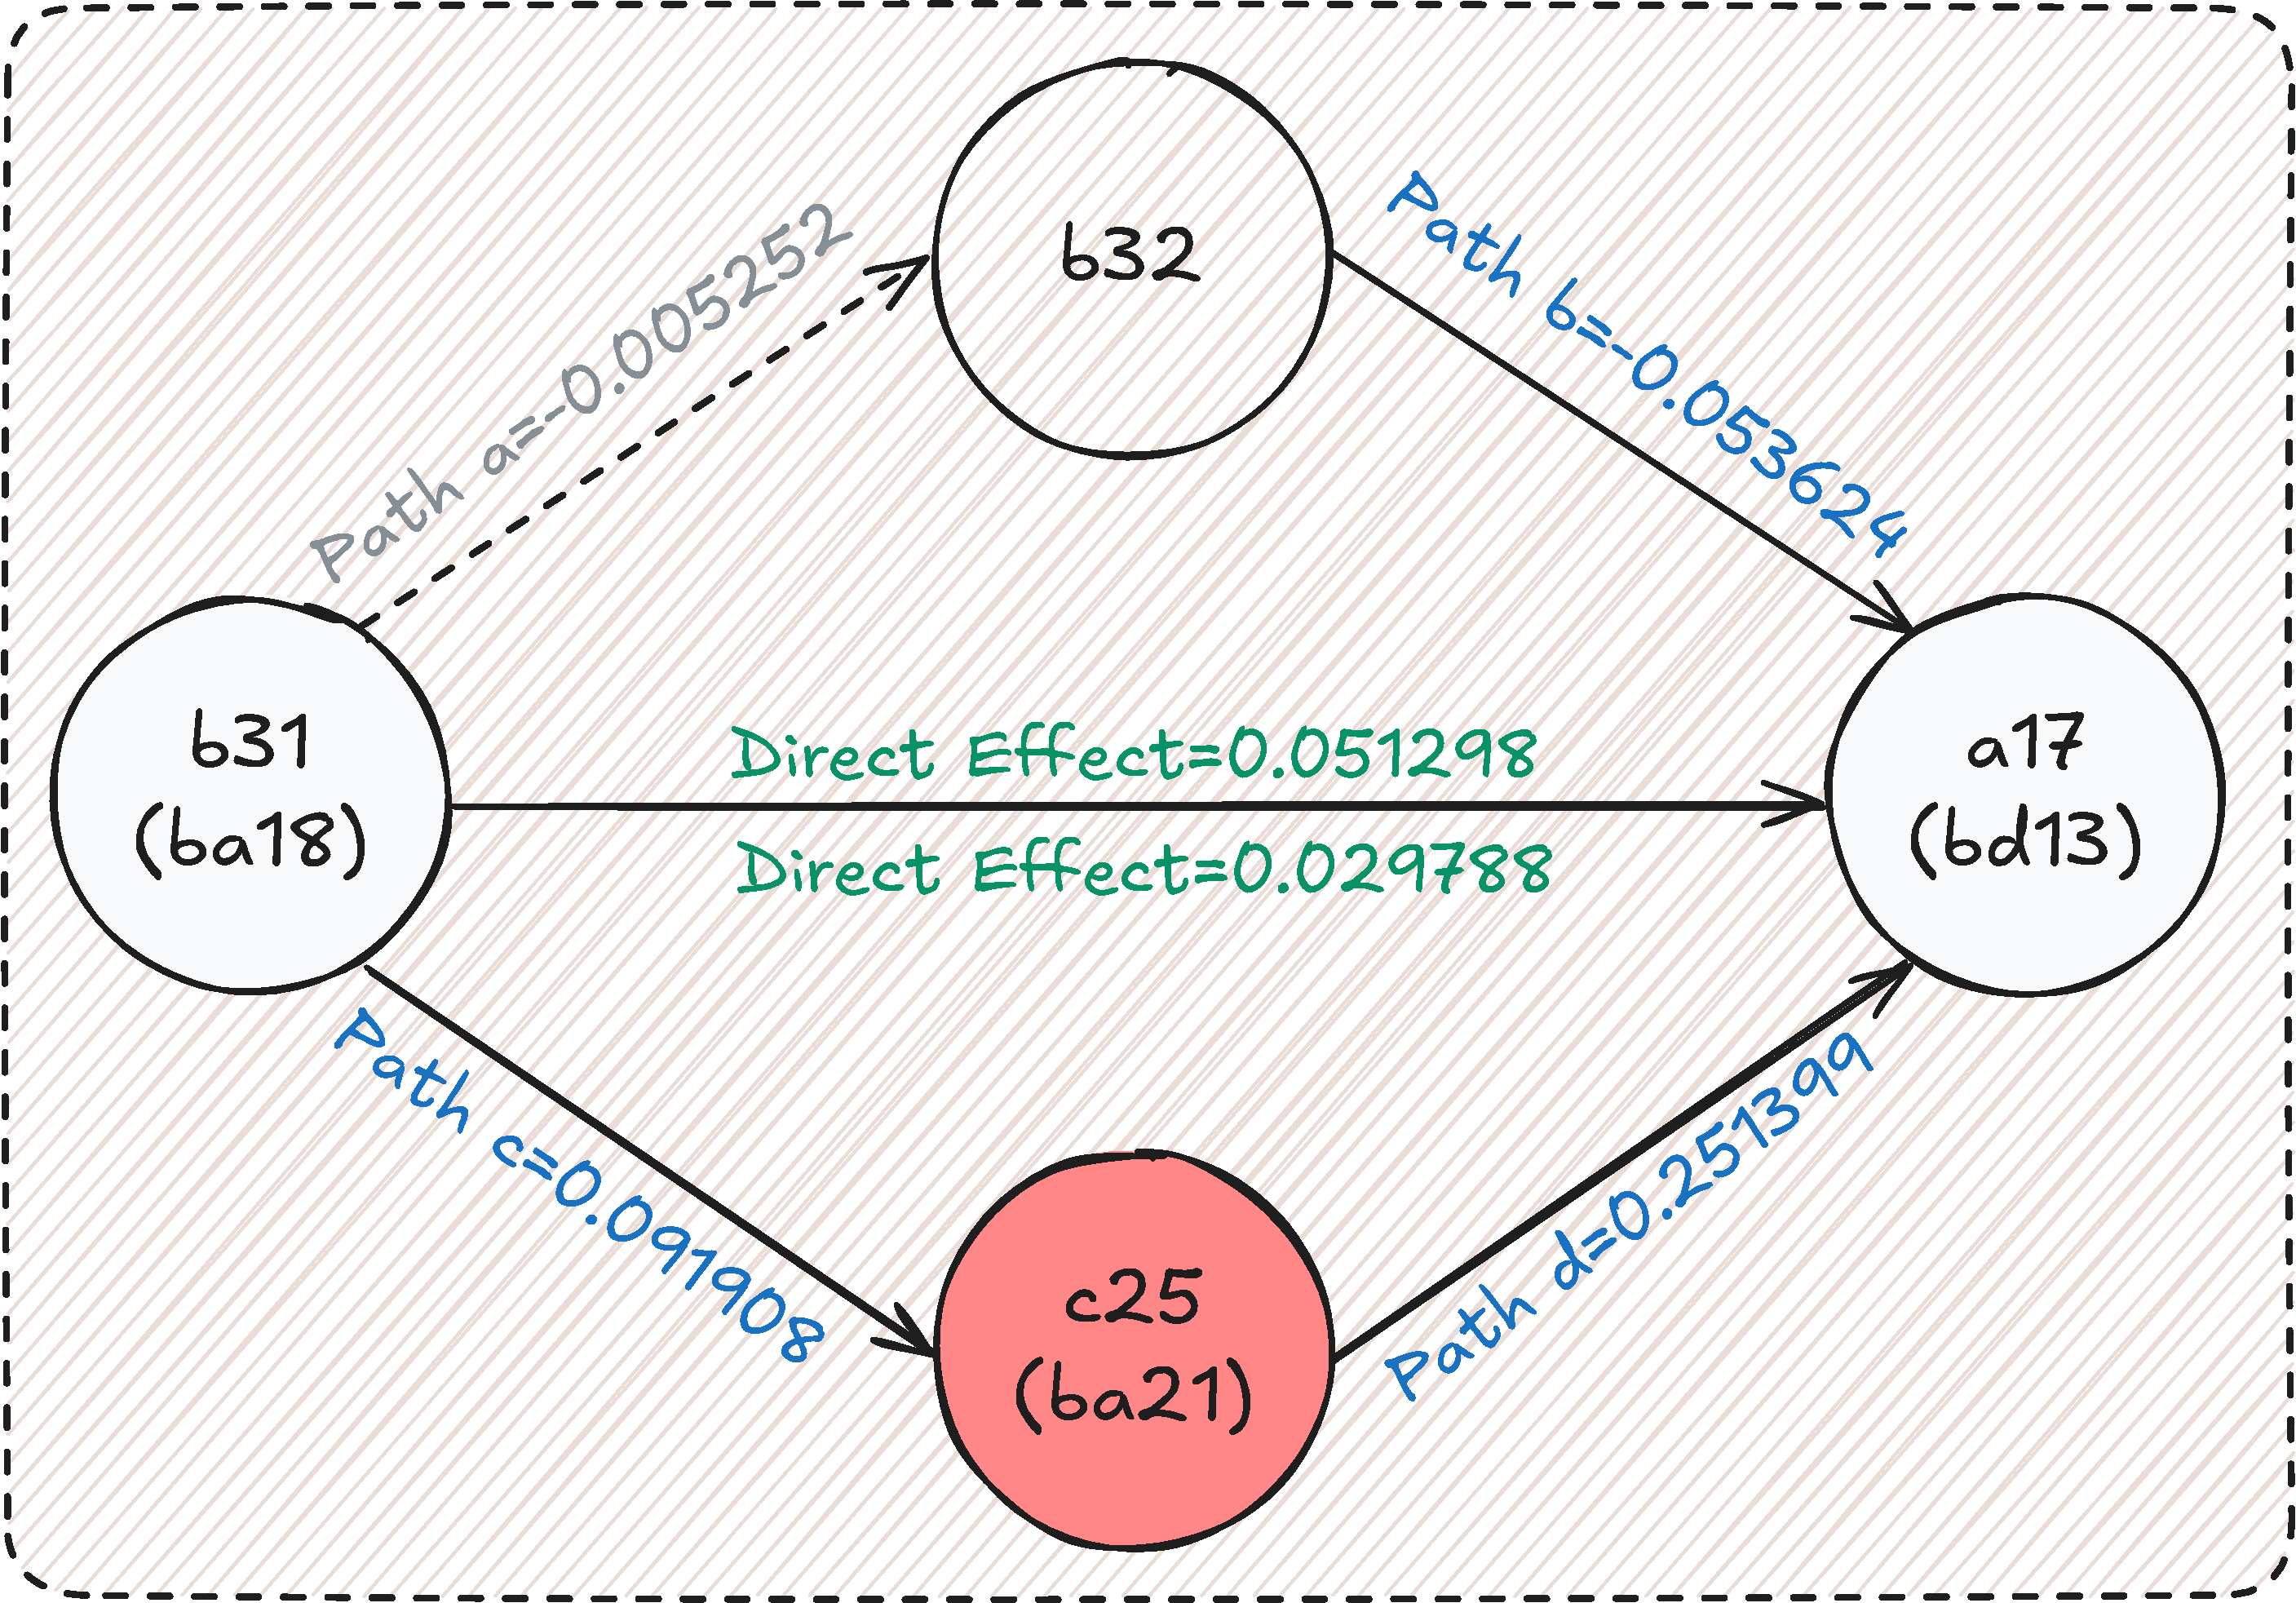
\includegraphics[width=0.7\linewidth]{./figs/mediation-pressure.pdf}
    \caption{中介效应模型路径（仅下支为通路）}\label{figure-mediation}
\end{figure}

\begin{table}[htbp]
    \centering
    \setlength{\tabcolsep}{7pt}
    \renewcommand{\arraystretch}{1.5}
    \caption{中介效应分析结果}\label{table-mediation}
    \begin{threeparttable}
        % \resizebox{\textwidth}{!}{
            \begin{tabular}{cccccc}
                \bottomrule[1.5pt]
                \textbf{路径} & Coeff ($\beta$) & SE & $p$ & 95\% CI & Sig. \\
                \midrule[0.75pt]
                b31$\to$b32 & -0.005252 & 0.008645 & 5.435137e-01 & $(-0.022198\sim0.011694)$ & No \\
                b32$\to$a17 & -0.053624 & 0.009908 & 6.444972e-08 & $(-0.073047\sim-0.034201)$ & Yes \\
                b31$\to$a17 & 0.051298 & 0.006996 & 2.524923e-13 & $(0.037583\sim0.065012)$ & Yes \\
                Indirect & 0.000279 & 0.000496 & 5.696000e-01 & $(-0.000657\sim0.001336)$ & No \\
                Total & 0.051577 & 0.007010 & 2.100852e-13 & $(0.037834\sim0.065319)$ & Yes \\
                \addlinespace
                c31$\to$c25 & 0.091908 & 0.005213 & 4.687083e-68 & $(0.081689\sim0.102126)$ & Yes \\
                c25$\to$a17 & 0.251399 & 0.015805 & 5.997055e-56 & $(0.220416\sim0.282383)$ & Yes \\
                b31$\to$a17 & 0.029788 & 0.007059 & 2.476000e-05 & $(0.015950\sim0.043625)$ & Yes \\
                Indirect & 0.021789 & 0.002088 & 0.000000e+00 & $(0.018058\sim0.026252)$ & Yes \\
                Total & 0.051577 & 0.007010 & 2.100852e-13 & $(0.037834\sim0.065319)$ & Yes \\
                \toprule[1.5pt]
            \end{tabular}
        % }
        \begin{tablenotes}\small
            \item 【注】Bootstrap 重采样次数为 5000 轮
        \end{tablenotes}
    \end{threeparttable}
\end{table}

重采样次数为 5000 次，分别检验“学业期望压力”与“未来信心水平”在家庭教育期望与青少年心理健康之间的中介作用，图~\ref{figure-mediation} 显现了下分支是通路，上分支 $\text{b31}\to\text{b32}$ 路径不显著，因此为虚线，链路失效。表~\ref{table-mediation} 可得如下结论：

\noindent$\blacktriangleright$ \textbf{学业期望压力中介}

\begin{itemize}
    \item 父母教育期望（b31）对学业期望压力（b32）的路径系数不显著（$\beta=-0.005,\ p=0.544>0.05$）；
    \item 虽然学业期望压力对青少年心理健康水平（a17）具有显著的负向预测作用（$\beta=-0.054,\ p<0.001$），但中介效应的 Bootstrap 95\% 置信区间（95\% $\text{CI}=-0.000657\sim0.001336$）包含 0 点。
\end{itemize}

根据这一分析结果，表明了“父母教育期望 $\to$ 学业成绩压力 $\to$ 青少年初中生心理健康”这一中介路径不成立。

\noindent$\blacktriangleright$ \textbf{未来信心水平中介}

\begin{itemize}
    \item 教育期望（c31）显著正向预测个体的未来信心水平（$\beta=0.092,\ p<0.001$）；
    \item 未来信心水平显著正向预测其心理健康水平（$\beta=0.251,\ p<0.001$）；
    \item 在控制了中介变量后，教育期望对心理健康水平的直接效应（$\beta=0.030,\ p<0.001$）依然显著。
\end{itemize}

中介效应检验分析表明，未来信心水平的中介效应值为 0.022，且 Bootstrap 95\% 置信区间不包含 0 点（$0.018058\sim0.026252$），占总效应 0.052 的比重约为 42.3\%，这蕴含着对未来信心水平在家庭教育期望影响青少年初中生心理健康过程中起到了显著的部分中介作用。



\section{结论}
本研究基于中国教育追踪调查 CEPS 数据集，筛选出 6891 名七年级青少年初中生及其家长作为有效样本，系统探讨了家庭教育期望对初中生心理健康的影响。通过描述性统计、差异性检验、多元线性回归及中介效应模型分析，本课程论文研究揭示了家庭期望与青少年心理健康之间复杂的动态关系，主要研究结论概括如下：

\paragraph*{a) 家庭教育期望与心理健康现状及分布特征}~{}

\begin{itemize}
    \item \textbf{期望普遍较高与代际偏差并存：}数据显示，多数家长（约 37.47\%）期望子女获得大学本科学历，且“家长期望高于子女期望”的现象（约 33.71\%）在汉族家庭中显著多于“家长期望低于子女期望”，这表明家长普遍扮演高标准制定者的角色，且对男生的学业施压期望偏差显著高于女生。
    \item \textbf{家庭资源与期望一致性的正相关：}家庭经济条件越好、拥有独立书桌等学习资源的家庭，亲子间教育期望的一致性越高，这说明优渥的物质基础有助于缓解家庭内部焦虑，促进亲子在学业目标上的共识。
\end{itemize}

\paragraph*{b) 人口学特征与家庭背景的显著差异性}~{}

\begin{itemize}
    \item \textbf{群体差异显著：}独立样本 $t$ 检验显示，男生、独生子女、拥有独立书桌、参加辅导班以及非低保家庭的学生，其心理健康水平显著更高，值得注意的是，尽管男生面临更高的家庭期望压力，但其心理健康得分在统计上略高于女生（$\mu_{\text{男}}=4.146$ vs. $\mu_{\text{女}}=4.095$），尽管实际效应量微弱（Cohen's $d=-0.057$）。
    \item \textbf{经济地位的阶梯效应：}单因素方差分析 ANOVA 说明，随着家庭经济条件的改善，青少年心理健康水平呈上升趋势，但在达到“比较富裕”水平后，这种增益趋于收敛。
    \item \textbf{家长投入的积极作用：}家长为孩子付出程度与心理健康呈正相关，尤其是当付出程度达到“比较多”或“非常多”时，对子女心理健康的促进作用尤为显著。
\end{itemize}

\paragraph*{c) 心理健康的核心预测因素信心胜于压力}~{}

\begin{itemize}
    \item \textbf{自我信心是核心保护因子：}相关性分析与回归分析一致表明，学生对未来的信心水平是其心理健康最强有力的正向预测因子（$\lambda=0.2138,\ p<0.001$）。
    \item \textbf{家长信心的传递效应：}家长对孩子未来的信心比单纯的学业成绩要求更能预测孩子的心理健康（$\lambda=0.1647,\ p<0.001$），家长的高信心能够转化为孩子的心理资本，而单纯的高学业要求虽有正向关联，但影响力较弱。
    \item \textbf{学业压力的负面影响：}学业期望带来的压力与心理健康呈显著负相关，感到“压力很大”的学生心理健康水平显著下降。
\end{itemize}

\paragraph*{d) 家庭期望影响心理健康的内在机制验证}~{}

\begin{itemize}
    \item \textbf{“对未来信心水平”起部分中介作用：}这是一个关键的积极路径，家长较高的教育期望能够显著提升青少年对未来的信心（$\beta=0.092$），进而显著提升其心理健康水平（$\beta=0.251$），该中介效应占总效应的 42.3\%，Bootstrap 95\% 置信区间为 $(0.018\sim0.026)$，不包含 0 点，证明了适度的高期望能通过激发内在动力来促进心理健康。
    \item \textbf{“学业期望压力”中介路径不成立：}尽管学业压力直接负向影响心理健康，但在本研究模型中，家庭教育期望并未显著直接导致青少年七年级学生学业压力的增加（路径系数 $p>0.05$），因此“家长期望 $\rightarrow$ 学业压力 $\rightarrow$ 心理健康”这一中介假设未获支持，这提示我们，家庭教育期望本身并不必然转化为负面压力，压力的产生可能更多源于青少年学生对要求的内化程度或缺乏支持系统。
\end{itemize}

\vspace*{1em}

综上所述，家庭教育期望对七年级青少年初中生的心理健康具有双重影响。一方面，基于信任与支持的高期望能通过增强青少年的未来信心，发挥积极的保护作用；另一方面，脱离实际的高压环境若导致学生信心缺失，则会损害心理健康。本文建议家长在家庭教育中应注重“信心支持”而非单纯的“指标施压”，致力于缩进亲子间的期望偏差，构建和谐的沟通机制，与此同时，我们尤其需要关注经济困难家庭及缺乏独立学习空间的青少年学生群体，通过提供情感支持和资源倾斜，通过提升其自我效能感，来维护他们的心理健康发展。












\clearpage
\cfoot{}
\setlength{\bibhang}{2em}
\renewcommand{\refname}{}
\centerline{\zihao{3}\bfseries\@参考文献}
\vspace*{-3em}

\begin{thebibliography}{32}\zihao{5}
    \bibitem[Walberg(1984)]{Walberg} Walberg, H. J. (1984). Families as partners in educational productivity. \textit{Phi delta kappan}, \textit{65}(6), 397--400.
    \bibitem[王亚楠(2024)]{WangYaNan} 王亚楠. (2024). 亲子间教育期望匹配对初中生学习投入的影响. 硕士学位论文, 青岛大学.
    \bibitem[Xu, Zuo, \& Zheng(2024)]{CEPS} Xu, T., Zuo, F., \& Zheng, K. (2024). Parental Educational Expectations, Academic Pressure, and Adolescent Mental Health: An Empirical Study Based on CEPS Survey Data. \textit{International Journal of Mental Health Promotion}, \textit{26}(2), 93--103.
    \bibitem[Bronfenbrenner(1979)]{Bronfenbrenner} Bronfenbrenner, U. (1979). \textit{The ecology of human development: Experiments by nature and design}. Harvard university press.
    \bibitem[Resnick et al.(1997)]{Resnick} Resnick, M. D., Bearman, P. S., Blum, R. W., Bauman, K. E., Harris, K. M., Jones, J., Tabor, J., Beuhring, T., Sieving, R. E., Shew, M., Ireland, M., Bearinger, L. H., \& Udry, J. R. (1997). Protecting adolescents from harm. Findings from the National Longitudinal Study on Adolescent Health. \textit{JAMA}, \textit{278}(10), 823--832.
    \bibitem[马汴京 \& 张元峰(2022)]{MaBianJing} 马汴京, \& 张元峰. (2022). 父母高教育期望与青少年心理健康——基于亲子间教育期望差异的视角. \itsongti{青年研究}, (05), 32-44+94-95.
    \bibitem[Chen \& Uttal(1988)]{Cultural} Chen, C., \& Uttal, D. H. (1988). Cultural Values, Parents' Beliefs, and Children's Achievement in the United States and China. \textit{Human Development}, \textit{31}(6), 351--358.
    \bibitem[Ma, Siu, \& Tse(2018)]{Role} Ma, Y., Siu, A., \& Tse, W. S. (2018). The role of high parental expectations in adolescents' academic performance and depression in Hong Kong. \textit{Journal of Family Issues}, \textit{39}(9), 2505--2522.
    \bibitem[李大林 et al.(2025)]{LiDaLin} 李大林, 吴强, 黄梅, 朱俊, 念靖晴, \& 吴文峰. (2025). 父母期望对高中生抑郁的影响：父母心理控制和学习压力的中介作用. \itsongti{中国临床心理学杂志}, \textit{33}(02), 261-266+271.
    \bibitem[Higgins(1987)]{Higgins} Higgins, E. T. (1987). Self-discrepancy: A theory relating self and affect. \textit{Psychological Review}, \textit{94}(3), 319--340.
    \bibitem[杨雪 \& 魏雅鑫(2024)]{YangXue} 杨雪, \& 魏雅鑫. (2024). 中国家庭教育期望的代际偏差与青少年发展. \itsongti{人口学刊}, \textit{46}(01), 53-66.
    \bibitem[郭筱琳, 何苏日那, 秦欢, 刘春晖, \& 罗良(2019)]{GuoXiaoLin} 郭筱琳, 何苏日那, 秦欢, 刘春晖, \& 罗良. (2019). 亲子间教育期望差异对小学生情感幸福感的影响：学业成绩和学业自我效能感的中介作用. \itsongti{心理发展与教育}, \textit{35}(04), 467--477.
    \bibitem[Fan \& Hui(2025)]{Burnout} Fan, X., \& Hui, A. N. N. (2025). Academic Burnout and Parent-Child Discrepancies in Educational Expectations Among Chinese Adolescents: A Moderated Mediation Model. \textit{Behavioral Sciences}, \textit{15}(7), 876.
    \bibitem[李文哲 \& 胡开(2025)]{LiWenZhe} 李文哲, \& 胡开. (2025). 高期望必然导致高抑郁？——基于亲子教育期望偏差视角及中介效应分析. \itsongti{当代青年研究}, (05), 100--116.
    \bibitem[张云运, 陈嘉仪, 杨妙, 任萍, \& 刘思辰(2021)]{ZhangYunYun} 张云运, 陈嘉仪, 杨妙, 任萍, \& 刘思辰. (2021). 父母学业参与、父母学业压力与青少年早期的学业投入：有调节的中介模型. \itsongti{心理发展与教育}, \textit{37}(02), 211--221.
    \bibitem[李若璇, 朱文龙, 刘红瑞, \& 姚梅林(2018)]{LiRuoXuan} 李若璇, 朱文龙, 刘红瑞, \& 姚梅林. (2018). 家长教育期望对学业倦怠的影响：家长投入的中介及家庭功能的调节. \itsongti{心理发展与教育}, \textit{34}(04), 489--496.
    \bibitem[熊茗伶, 王泉泉, 熊昱可, 江雯琪, \& 任萍(2024)]{XiongMingLing} 熊茗伶, 王泉泉, 熊昱可, 江雯琪, \& 任萍. (2024). 感知到父母施加的学业压力对不同性别青少年心理适应的影响：自我韧性的保护作用. \itsongti{心理发展与教育}, \textit{40}(04), 542--550.
    \bibitem[程雅雯, 闫思宇, \& 杨钋(2025)]{ChengYaWen} 程雅雯, 闫思宇, \& 杨钋. (2025). 班级非独生子女比例与学生心理健康——基于中国教育追踪调查（CEPS）的实证研究. \itsongti{基础教育}, \textit{22}(02), 67-80+93.
    \bibitem[Xu, Liu, Tu, \& Yang(2025)]{Differences} Xu, G., Liu, Y., Tu, Z., \& Yang, X. (2025). A Study on the Differences in Parental Educational Expectations and Adolescents' Academic and Psychological Development: A Comparative Analysis of Only Children and Non-Only Children. \textit{Behavioral Sciences}, \textit{15}(4), 402.
    \bibitem[王建武 \& 王思杨(2025)]{WangJianWu} 王建武, \& 王思杨. (2025). 促进还是抑制：父母教育期望与投入对子女心理健康的影响. \itsongti{青年研究}, (03), 175-192+198.
    \bibitem[李佳哲, 王雪纯, \& 赵瑛瑛(2024)]{LiJiaZhe} 李佳哲, 王雪纯, \& 赵瑛瑛. (2024). 代际教育期望及其差异对城市初中生学业表现的影响——基于父母学历的异质性分析. \itsongti{教育科学研究}, (01), 51--59.
    \bibitem[Tichenor, Donohue, \& Olien(1970)]{Tichenor} Tichenor, P. J., Donohue, G. A., \& Olien, C. N. (1970). Mass Media Flow and Differential Growth in Knowledge. \textit{The Public Opinion Quarterly}, \textit{34}(2), 159--170.
    \bibitem[de Moivre(1733)]{Moivre} de Moivre, A. (1733). ``Approximatio ad Summam Terminorum Binomii $\displaystyle(a+b)^n$ in Seriem Expansi''. \textit{Self-published Pamphlet}, \textit{7}.
    \bibitem[P\'olya(1920)]{Polya} P\'olya, G. (1920). \"Uber den zentralen Grenzwertsatz der Wahrscheinlichkeitsrechnung und das Momentenproblem. \textit{Math Z}, \textit{8}, 171--181.
    \bibitem[Pearson(1896)]{Pearson} Pearson, K. (1896). Mathematical Contributions to the Theory of Evolution. III. Regression, Heredity, and Panmixia. \textit{Philosophical Transactions of the Royal Society of London}. \textit{Series A}, \textit{187}, 253--318.
    \bibitem[Legendre(1805)]{Legendre} Legendre, A. M. (1805). \textit{Nouvelles m{\'e}thodes pour la d{\'e}termination des orbites des com{\`e}tes}. France: F. Didot.
\end{thebibliography}

\end{document}